{\centering
	\chapter{Construction}\label{parte2}}
\thispagestyle{empty}
\noindent
\begin{minipage}[t]{0.35\textwidth}
	\begin{flushright}
		\large
		\vspace{1pt}
		三十輻共一轂，\\
		當其無，有車之用。\\
		\vspace{0.5em}
		埏埴以為器，\\
		當其無，有器之用。\\
		\vspace{0.5em}
		鑿戶牖以為室，\\
		當其無，有室之用。\\
		\vspace{0.5em}
		故有之以為利，\\
		無之以為用。
	\end{flushright}
\end{minipage}%
\hfill
\vrule width 0.5pt % La línea vertical
\hfill
\begin{minipage}[t]{0.55\textwidth}
	\vspace{1pt}
	\raggedright
	\emph
	Thirty spokes converge to form a wheel hub.\\
	But it is the emptiness inside the hub that makes it useful.\\
	
	\vspace{0.8em}
	Clay is kneaded to form a pot.\\
	But it is the emptiness inside it that makes it useful.\\
	
	\vspace{0.8em}
	Doorways and window bays are chiselled to form a house.\\
	But it is the emptiness inside it that makes it useful.\\

	\vspace{0.8em}
	Substance brings benefits.\\
	Emptiness brings usefulness.
\end{minipage}

\vspace{1em}
\hfill {\normalfont  道德經 —\textsc{Dàodé Jīng, Chapter 11}}

\section{Go in two dimensions and two players.}

Let us interpret the board in a convenient manner by considering solely its points of intersection. Let \(n, m \in \mathbb{N}\). We define \(N = \{1, \dots, n\}\) and \(M = \{1, \dots, m\}\). With these sets, we formalize the game space:\footnote{We use the letter \(G\) because we will adopt Japanese Go terminology for our notation whenever it does not lead to confusion. In Japanese, the board is called \textit{Goban} (碁盤).}
$$  G \coloneqq N \times M = \{(x,y) : x \in N,\, y \in M\}.  $$

Let $t_1, t_2 \in G$ be two \textit{points}\footnote{The letter $t$ originates from the term \textit{ten} (点), meaning point in Japanese (and Chinese).}. If $t_1=(a,b)$, we say that $t_2$ is adjacent to $t_1$, denoted by $t_1 \sim t_2$, if it satisfies exactly one of the following conditions:
$$t_2 = (a+1,b), \quad t_2 = (a,b+1), \quad t_2 = (a-1,b), \quad t_2 = (a,b-1).$$

If none of these conditions hold, $t_1$ is not adjacent to $t_2$, which we denote by $t_1 \nsim t_2$. Figure~\ref{fig:Fig 13} illustrates the adjacencies of a point.

\begin{figure}[H]
	\centering
	\begin{tikzpicture}[scale=0.485] \tikzstyle{every node}=[font=\small]
		% Draw the background
		\fill[goban] (-0.5,-0.5) rectangle (6.5,6.5);
		
		% Draw the grid lines
		\draw[step=1cm, black] (0,0) grid (6,6);
		
		% Draw the thick border
		\draw[very thick] (0,0) rectangle (6,6);
		
		% Draw the central black dot
		\filldraw[black] (3,3) circle (4pt);
		
		\fill[Blue] (3.75,3.75) rectangle (4.25,4.25);
		\fill[OliveGreen] (3,4) circle (5pt);
		\fill[OliveGreen] (5,4) circle (5pt);
		\fill[OliveGreen] (4,3) circle (5pt);
		\fill[OliveGreen] (4,5) circle (5pt);
	\end{tikzpicture}
	\caption{Point \((5,5)\) in \textcolor{Blue}{blue}, adjacencies in \textcolor{OliveGreen}{green}.}
	\label{fig:Fig 13}
\end{figure}

Having established the \textit{where}, let us examine \textit{who} participates in it. When reviewing the rules, we observed that each point on the board can be in one of three possible states: unoccupied, occupied by a white stone, or occupied by a black stone. We define \(E\) as the set of states that a point may assume:
$$E=\{0,1,2\}.$$
These values represent, respectively: vacant, black, and white. With this, we can account for all possible states on the board:
\begin{align*}
	E \times G &= \{(e,t) : e \in E, t \in G \}.
\end{align*}
For example, the point \((4,4) \in G\) may be found in one of three states: \((0,(4,4))\), meaning no stone at \((4,4)\); \((1,(4,4))\), a black stone at \((4,4)\); or \((2,(4,4))\), a white stone at \((4,4)\).


We shall refer to the elements of \(E \times G\) as \textit{stones}, denoted by the letter \(i\), such that \(i=(e,t)\),\footnote{From the term \textit{ishi} (石), meaning ``stone'' in Japanese.} with \(e \in E\) and \(t \in G\). In Go, however, a single point cannot exhibit all states simultaneously; it assumes at most one.

\begin{definition}[Board]
	A subset \(T \subseteq E \times G\) is said to be a \textit{board} if, given \((e,t) \in T\),
	$$(e',t) \notin T, \quad \forall e' \neq e.$$

\end{definition}

That is, in $T$ there is a unique state for each position. Having established the \textit{where} and \textit{who}, we can construct the \textit{what}. To do so, we require two fundamental functions:

\begin{definition}[Stone State Function]
	\label{funcioncolor}$$\text{We define } C: E \times G \to E, \quad (e,t) \mapsto e.$$
	\end{definition}
	
\begin{definition}[Stone Position Function]
	\label{funcionposiciion}$$\text{We define } P: E \times G \to G, \quad (e,t) \mapsto t.$$
	\end{definition}
	
Equipped with these, the notion of a group arises naturally:

\begin{definition}[Connection]Let $T$ be a board and let $i_1, i_2 \in T$ be two stones. We say that $i_1$ and $i_2$ are connected, denoted by $i_1 \leftrightarrow i_2$, if
	$$C(i_1) = C(i_2) \quad \text{and} \quad P(i_1) \sim P(i_2).$$
\end{definition}


\begin{definition}[Group of Stones]
	Given a board $T$, two stones $i_a$ and $i_b$ belong to the same group (denoted by $i_a \equiv i_b$) if there exists a finite sequence of stones $\{i_1, i_2, \dots, i_k\}$ such that $i_1 = i_a$, $i_k = i_b$, and each stone is connected to the next ($i_m \leftrightarrow i_{m+1}$). The relation $\equiv$ is an equivalence relation.
	
	We shall denote groups by \(I^e\), where \(e\) designates the state or color of the group; alternatively, we may write ``\textit{Let \(I\) be a group of color \(e\)},'' or simply \(I\) whenever the color is not relevant.\footnote{From \textit{ishi} (石, stone/stones). Denoted similarly to individual stones, but capitalized to signify a set thereof.}
\end{definition}
	

\begin{definition}[Adjacencies of a Group]
	Let $I$ be a group of color $e$, and let $i=(e',t)$ be a stone on the board. We say that $I$ is adjacent to $i$, denoted by $I \sim i$, if at least one stone in the group is adjacent to $i$:
	$$I \sim i \iff \exists \ i_k \in I : P(i_k) \sim P(i).$$
\end{definition}

These definitions likewise encompass the groups $I^{0}$. Given their fundamental importance, these groups are given a dedicated name: we shall refer to them as \textit{regions} and denote them simply by the letter $R$.

To refer to the color of a group as a whole, we define \(C(I^{e}) = e\), by virtue of the fact that all of its constituent elements share the same state.

\begin{wrapfigure}[13]{r}{0.35\textwidth}
	%\begin{figure}[H]
	\centering
	\begin{tikzpicture}[scale=0.485] \tikzstyle{every node}=[font=\small]
		% Draw the background
		\fill[goban] (-0.5,-0.5) rectangle (6.5,6.5);
		
		% Draw the grid lines
		\draw[step=1cm, black] (0,0) grid (6,6);
		
		% Draw the thick border
		\draw[very thick] (0,0) rectangle (6,6);
		
		% Draw the central black dot
		
		\filldraw[black] (2,4) circle (12pt);
		\filldraw[black] (3,4) circle (12pt);
		\filldraw[black] (4,3) circle (12pt);
		\filldraw[black] (4,4) circle (12pt);
		\filldraw[draw=black,fill=white] (3,3) circle (12pt);
		\filldraw[draw=black,fill=white] (3,2) circle (12pt);
		\fill[OliveGreen] (3,3) circle (5pt);
		\fill[OliveGreen] (1,4) circle (5pt);
		\fill[OliveGreen] (5,4) circle (5pt);
		\fill[OliveGreen] (3,5) circle (5pt);
		\fill[OliveGreen] (2,5) circle (5pt);
		\fill[OliveGreen] (4,5) circle (5pt);
		\fill[OliveGreen] (4,2) circle (5pt);
		\fill[OliveGreen] (2,3) circle (5pt);
		\fill[OliveGreen] (5,3) circle (5pt);
		
	\end{tikzpicture}
	\caption{A black group with its \textcolor{OliveGreen}{adjacencies} marked.}
	\label{ejemplo_adyacencias}
\end{wrapfigure}
It will prove very useful to identify the adjacencies of a stone or group. To this end, we define the set \(K\)\footnote{From the term \textit{chikaku} (近く, near/nearby).} associated with a stone or group (see Figure~\ref{ejemplo_adyacencias}).


\begin{definition}[Adjacency Set]
	Let \(i\) be a stone and let \(I\) be a group of stones of color \(e\). We define the adjacency set of the stone as the stones satisfying the definition of adjacency, namely:
	$$K(i) = \{i_r : P(i) \sim P(i_r)\}.$$
	Analogously, for a group $I$, we define:
	$$K(I) = \{i_r : I \sim i_r\}.$$
\end{definition}


Note that any adjacent stone of the same color already belongs to the group. Thus, if the group is of color $e$, the states of its adjacencies will belong, at most, to $E \setminus \{e\}$.

To characterize the states of these adjacencies, we will make use (and abuse) of the functions previously defined.

\begin{definition}[State of the Adjacencies of a Group or Stone]\label{def_estados}
	Let $I$ be a group of color $e$. Applying the function $C$ elementwise to its adjacency set $K(I)$, we obtain the intended set, defined as:
	$$C(K(I)) = \{C(i) \mid i \in K(I)\} \subseteq \{0, e'\}.$$
	Analogously, for an individual stone $i = (e,t)$, we define:
	$$C(K(i)) = \{C(i_k) \mid i_k \in K(i)\} \subseteq \{0, e'\}.$$
	\end{definition}

This definition is essential for describing much of the internal dynamics of Go. Henceforth, whenever we refer to groups $I$, it is to be understood that their color is distinct from $0$. Whenever we deal with $I^{0}$, we shall employ the notation $R$, unless explicitly stated otherwise.

\begin{wrapfigure}[11]{r}{0.35\textwidth}
	\vspace{-36pt}
	\centering
	\begin{tikzpicture}[scale=0.485] \tikzstyle{every node}=[font=\small]
		% Draw the background
		\fill[goban] (-0.5,-0.5) rectangle (6.5,6.5);
		
		% Draw the grid lines
		\draw[step=1cm, black] (0,0) grid (6,6);
		
		% Draw the thick border
		\draw[very thick] (0,0) rectangle (6,6);
		
		% Draw the central black dot
		\filldraw[draw=black,fill=white] (2,3) circle (12pt);
		\filldraw[draw=black,fill=white] (1,3) circle (12pt);
		\filldraw[draw=black,fill=white] (3,3) circle (12pt);
		\filldraw[draw=black,fill=white] (1,5) circle (12pt);
		\filldraw[draw=black,fill=white] (1,4) circle (12pt);
		\filldraw[draw=black,fill=white] (4,2) circle (12pt);
		\filldraw[draw=black,fill=white] (4,1) circle (12pt);
		\filldraw[draw=black,fill=white] (4,0) circle (12pt);
		\filldraw[draw=black,fill=white] (0,5) circle (12pt);
		\filldraw[black] (5,3) circle (12pt);
		\filldraw[black] (5,4) circle (12pt);
		\filldraw[black] (4,4) circle (12pt);
		\filldraw[black] (3,4) circle (12pt);
		\filldraw[black] (2,5) circle (12pt);
		\filldraw[black] (2,6) circle (12pt);
		\filldraw[black] (5,2) circle (12pt);
		\filldraw[black] (5,1) circle (12pt);
		\filldraw[black] (5,0) circle (12pt);
		
		\filldraw[Blue] (0,0) circle (6pt);
		\filldraw[Blue] (0,1) circle (6pt);
		\filldraw[Blue] (0,2) circle (6pt);
		\filldraw[Blue] (0,3) circle (6pt);
		\filldraw[Blue] (0,4) circle (6pt);
		\filldraw[Blue] (1,0) circle (6pt);
		\filldraw[Blue] (1,1) circle (6pt);
		\filldraw[Blue] (1,2) circle (6pt);
		\filldraw[Blue] (2,0) circle (6pt);
		\filldraw[Blue] (2,1) circle (6pt);
		\filldraw[Blue] (2,2) circle (6pt);
		\filldraw[Blue] (3,0) circle (6pt);
		\filldraw[Blue] (3,1) circle (6pt);
		\filldraw[Blue] (3,2) circle (6pt);
		
		\filldraw[OliveGreen] (6,6) circle (6pt);
		\filldraw[OliveGreen] (6,5) circle (6pt);
		\filldraw[OliveGreen] (6,4) circle (6pt);
		\filldraw[OliveGreen] (6,3) circle (6pt);
		\filldraw[OliveGreen] (6,2) circle (6pt);
		\filldraw[OliveGreen] (6,1) circle (6pt);
		\filldraw[OliveGreen] (6,0) circle (6pt);
		\filldraw[OliveGreen] (5,6) circle (6pt);
		\filldraw[OliveGreen] (4,6) circle (6pt);
		\filldraw[OliveGreen] (3,6) circle (6pt);
		\filldraw[OliveGreen] (5,6) circle (6pt);
		\filldraw[OliveGreen] (4,6) circle (6pt);
		\filldraw[OliveGreen] (3,6) circle (6pt);
		\filldraw[OliveGreen] (5,5) circle (6pt);
		\filldraw[OliveGreen] (4,5) circle (6pt);
		\filldraw[OliveGreen] (3,5) circle (6pt);
		\filldraw[OliveGreen] (5,6) circle (6pt);
		\filldraw[OliveGreen] (4,6) circle (6pt);
		\filldraw[Orange] (0,6) circle (6pt);
		\filldraw[Orange] (1,6) circle (6pt);
		\filldraw[Orange] (2,4) circle (6pt);
		\filldraw[Orange] (4,3) circle (6pt);
		\filldraw[Blue] (0,0) circle (6pt);
	\end{tikzpicture}
	\caption{\textcolor{Blue}{White}, \textcolor{OliveGreen}{black}, and \textcolor{Orange}{neutral} territory.}
	\label{fig:territorios}
\end{wrapfigure}


\begin{definition}[Territory]
	A region \(R\) is territory belonging to the player of color \(e\) if there exists a set \(S\) of groups of color \(e\) such that
	$$ K(R) \subseteq \bigcup_{I\in S} I. $$
\end{definition}

That is to say, all stones adjacent to the region belong to groups of the same color. We shall denote the \textit{territories}\footnote{From the term \textit{ji} (地), meaning ``land'' in Japanese.} of each color as:
$$J^{e} = \{R : C(K(R)) = \{e\}\}, \quad e \neq 0.$$
Regions that do not constitute territory for either player will be denoted and defined as
$$J^{0}\coloneqq \{R : |C(K(R))| \geq 2\}.$$

Figure~\ref{fig:territorios} illustrates the different types of \textit{territories}.


With this, we have established a partition of the set of \textit{regions} ($I^{0}$), since every region belongs to White's territory, belongs to Black's territory, or forms part of neither player's territory:
\begin{align*}
	I^{0} = J^{0} \cup J^{1} \cup J^{2}.
\end{align*}
\label{posicion_espacial}
Additionally, the cardinality of the adjacency set of an individual stone, $|K(i)|$\footnote{This is exactly as the degree of a vertex in graph theory.}, proves remarkably useful for determining its spatial placement on the board. Because $|K(i)|$ is bounded by Lemma~\ref{lem:2n}, a straightforward analysis of the number of adjacencies reveals precisely whether the stone is situated in the interior, on an edge, or in a corner. This geometric property will be essential, and we shall make use of it in Sections~\ref{teoremas_go1} and~\ref{sec_JR}.

To formalize captures, we first introduce the concept of a \textit{liberty}.

\begin{definition}[Liberties of a Group]
	Let \(I\) be a group. We define the set of liberties of said group as:
	$$L(I) = \{i \in K(I) : C(i) = 0\}.$$
	\end{definition}

Note that if $L(I) = \varnothing$ for a given group, then that group is considered \textit{dead}. This situation can only occur upon executing a move and effecting a capture. But what constitutes a capture? What is a move?

A group is captured when it loses all of its liberties. Captured stones are removed from the board\footnote{We employ Chinese rules for scoring; if another ruleset is used, such as the Japanese one, a point would be awarded for each captured stone.}.

\begin{definition}[Capture Criterion]
	Let $I$ be a group; then,
	$$I \text{ is captured} \iff L(I) = \varnothing.$$
	To formalize the removal of these stones from the board, if \(I = \{i_1, i_2, \dots, i_n\}\), it suffices to reassign their states by setting \(C(i_j) = 0\) for all \(j=1, \dots, n\).
\end{definition}

We favor the phrasing \textit{is captured}, since death is the consequence of a capture.

\section{Toward Movement}

Thus far, we have described the static structure of the board. To model a game, we must incorporate the temporal evolution of play. To this end, we first define the space of all possible moves, which we denote by \(\mathcal{J}\):
$$\mathcal{J} \coloneqq \left((E \setminus \{0\}) \times G\right) \cup \{\varnothing\}.$$

\subsection{Move Function}\label{criterio_jugada}
When playing Go on our turn, we rather take a stone and place it on the board, or else we pass. We define the move function as $f: \mathbb{N} \to \mathcal{J}$. Let us examine an example.
\begin{wrapfigure}[4]{r}{0.4\textwidth}
	%\begin{figure}[H]
	\centering
	\begin{tikzpicture}[scale=0.485] \tikzstyle{every node}=[font=\small]
		
		% Draw the background
		\fill[goban] (-0.5,-0.5) rectangle (6.5,6.5);
		
		% Draw the grid lines
		\draw[step=1cm, black] (0,0) grid (6,6);
		
		% Draw the thick border
		\draw[very thick] (0,0) rectangle (6,6);
		
		% Draw the central black dot
		\filldraw[black] (2,2) circle  (4pt) ;
		\path (2,2) node [white]{1} ;
		
		\filldraw[black] (2,2) circle (12pt);
		\path (2,2) node [white]{1} ;
		
		\filldraw[black] (2,3) circle (12pt);
		\path (2,3) node [white]{3} ;
		
		\filldraw[black] (3,3) circle (12pt);
		\path (3,3) node [white]{5} ;
		
		\filldraw[black] (4,5) circle (12pt);
		\path (4,5) node [white]{7} ;
		
		\filldraw[black] (3,5) circle (12pt);
		\path (3,5) node [white]{9} ;
		
		\filldraw[draw=black,fill=white] (4,4) circle (12pt);
		\path (4,4) node [black]{2} ;
		\filldraw[draw=black,fill=white] (4,2) circle (12pt);
		\path (4,2) node [black]{4} ;
		\filldraw[draw=black,fill=white] (3,2) circle (12pt);
		\path (3,2) node [black]{6} ;
		\filldraw[draw=black,fill=white] (4,3) circle (12pt);
		\path (4,3) node [black]{8} ;
		\filldraw[draw=black,fill=white] (2,1) circle (12pt);
		\path (2,1) node [black]{10} ;
		\filldraw[draw=black,fill=white] (1,2) circle; 
	\end{tikzpicture}
\end{wrapfigure} \begin{align*}
	f(1) &= (1,(2,2)), & f(2) &= (1,(4,4)), & f(3) &= (1,(2,3)),\\
	f(4) &= (2,(4,2)), & f(5) &= (2,(3,3)), & f(6) &= (2,(3,2)),\\
	f(7) &= (1,(4,5)), & f(8) &= (1,(3,4)), & f(9) &= (1,(3,5)),\\
	f(10) &= (2,(2,1)), & f(11) &= \varnothing, & f(12) &= \varnothing.
\end{align*}
%\vspace{2.5cm} 
\break

\subsection{Rules of a Legal Move}
\begin{wrapfigure}[12]{r}{0.5\textwidth}
	\vspace{-15pt}
	%\begin{figure}[H]
	\centering
	\begin{tikzpicture}[scale=0.485] \tikzstyle{every node}=[font=\small]
		% Draw the background
		\fill[goban] (-0.5,-0.5) rectangle (6.5,6.5);
		% Draw the grid lines
		\draw[step=1cm, black] (0,0) grid (6,6);
		% Draw the thick border
		\draw[very thick] (0,0) rectangle (6,6);
		% Draw the central black dot
		\filldraw[black] (3,3) circle (4pt);
		
		\filldraw[draw=black,fill=black] (4,4) circle (12pt);
		\filldraw[draw=black,fill=black] (4,2) circle (12pt);
		\filldraw[draw=black,fill=black] (3,2) circle (12pt);
		\filldraw[draw=black,fill=black] (3,3) circle (12pt);
		\filldraw[draw=black,fill=black] (5,2) circle (12pt);
		\filldraw[draw=black,fill=black] (6,3) circle (12pt);
		\filldraw[draw=black,fill=white] (5,3) circle (12pt);
		\filldraw[draw=black,fill=black] (5,4) circle (12pt);
		\fill[draw=black,fill=BlueViolet, very thin] (3.75,2.75) rectangle (4.25,3.25);
		\path (3,7.25) node [black,very thick]{\large{White plays}} ;
		
		
		\begin{scope}[xshift=8cm]
			% Draw the background
			\fill[goban] (-0.5,-0.5) rectangle (6.5,6.5);
			% Draw the grid lines
			\draw[step=1cm, black] (0,0) grid (6,6);
			% Draw the thick border
			\draw[very thick] (0,0) rectangle (6,6);
			% Draw the central black dot
			\filldraw[black] (3,3) circle (4pt);
			
			\filldraw[draw=black,fill=white] (4,4) circle (12pt);
			\filldraw[draw=black,fill=white] (4,2) circle (12pt);
			\filldraw[draw=black,fill=white] (3,2) circle (12pt);
			\filldraw[draw=black,fill=white] (3,3) circle (12pt);
			\filldraw[draw=black,fill=white] (5,2) circle (12pt);
			\filldraw[draw=black,fill=white] (6,3) circle (12pt);
			\filldraw[black] (5,3) circle (12pt);
			\fill[draw=black,fill=BlueViolet, very thin] (3.75,2.75) rectangle (4.25,3.25);
			\filldraw[draw=black,fill=white] (5,4) circle (12pt);
			\path (3,7.25) node [black,very thick]{\large{Black plays}} ;
		\end{scope}
		
	\end{tikzpicture}
	\caption{In \textcolor{BlueViolet}{purple}, illegal moves, as they lead to suicide.}
	\label{sui_ej}
\end{wrapfigure}
The function records the moves, but not their legality. Lets analyze the rules. The \textit{suicide rule} prohibits placing a stone if doing so results in the immediate capture of one's own group (Figure~\ref{sui_ej}). There exists a single exception: a move played with no liberties is legal if it simultaneously captures a group of the opposite color (see Figure~\ref{fig: fig1.19}). Note that, due to this mechanic, when it is Black's turn, only white groups may be captured, and vice versa.\break 


\begin{wrapfigure}[11]{r}{0.5\textwidth}
	\vspace{-12pt}
	%\begin{figure}[H]
	\centering
	\begin{tikzpicture}[scale=0.485] \tikzstyle{every node}=[font=\small]
		% Draw the background
		\fill[goban] (-0.5,-0.5) rectangle (6.5,6.5);
		
		% Draw the grid lines
		\draw[step=1cm, black] (0,0) grid (6,6);
		
		% Draw the thick border
		\draw[very thick] (0,0) rectangle (6,6);
		
		% Draw the central black dot
		\filldraw[draw=black,fill=white] (3,4) circle (12pt);
		\filldraw[draw=black,fill=white] (2,3) circle (12pt);
		\filldraw[draw=black,fill=white] (4,3) circle (12pt);
		\filldraw[draw=black,fill=white] (3,2) circle (12pt);
		\filldraw[black] (3,1) circle (12pt);
		\filldraw[black] (2,2) circle (12pt);
		\filldraw[black] (4,2) circle (12pt);
		\path (3,2) node [black]{1};
		\begin{scope}[xshift=8cm]
			% Draw the background
			\fill[goban] (-0.5,-0.5) rectangle (6.5,6.5);
			
			% Draw the grid lines
			\draw[step=1cm, black] (0,0) grid (6,6);
			
			% Draw the thick border
			\draw[very thick] (0,0) rectangle (6,6);
			
			% Draw the central black dot
			\filldraw[draw=black,fill=white] (3,4) circle (12pt);
			\filldraw[draw=black,fill=white] (2,3) circle (12pt);
			\filldraw[draw=black,fill=white] (4,3) circle (12pt);
			\filldraw[black] (3,3) circle (12pt);
			\filldraw[black] (3,1) circle (12pt);
			\filldraw[black] (2,2) circle (12pt);
			\filldraw[black] (4,2) circle (12pt);
			\path (3,3) node [white]{2};
		\end{scope}
	\end{tikzpicture}
	\caption{Position of a stone under apparent suicide that is legal because it captures.}
	\label{fig: fig1.19}
\end{wrapfigure}To evaluate a move, we first verify whether it results in a capture. If so, the move is legal. If it does not capture, we inspect its liberties: if it has none, it constitutes suicide and is therefore illegal; otherwise, it is legal. As noted in Section~\ref{primerreglako}, we must keep the \textit{ko rule} in mind. This rule forbids the immediate recapture of a single stone if doing so reverts the board state precisely to the position of the preceding turn (see Figure~\ref{regla_ko_ej}). \break

\vspace{15pt}
\begin{wrapfigure}[6]{r}{0.5\textwidth}
	\vspace{-12pt}
	%\begin{figure}[H]
	\centering
	\begin{tikzpicture}[scale=0.485] \tikzstyle{every node}=[font=\small]
		% Draw the background
		\fill[goban] (-0.5,-0.5) rectangle (6.5,6.5);
		
		% Draw the grid lines
		\draw[step=1cm, black] (0,0) grid (6,6);
		
		% Draw the thick border
		\draw[very thick] (0,0) rectangle (6,6);
		
		% Draw the central black dot
		\filldraw[draw=black,fill=white] (3,4) circle (12pt);
		\filldraw[draw=black,fill=white] (2,3) circle (12pt);
		\filldraw[draw=black,fill=white] (4,3) circle (12pt);
		\filldraw[draw=black,fill=white] (3,2) circle (12pt);
		\filldraw[black] (3,1) circle (12pt);
		\filldraw[black] (2,2) circle (12pt);
		\filldraw[black] (4,2) circle (12pt);
		\path (3,2) node [black]{1};
		\begin{scope}[xshift=8cm]
			% Draw the background
			\fill[goban] (-0.5,-0.5) rectangle (6.5,6.5);
			
			% Draw the grid lines
			\draw[step=1cm, black] (0,0) grid (6,6);
			
			% Draw the thick border
			\draw[very thick] (0,0) rectangle (6,6);
			
			% Draw the central black dot
			\filldraw[draw=black,fill=white] (3,4) circle (12pt);
			\filldraw[draw=black,fill=white] (2,3) circle (12pt);
			\filldraw[draw=black,fill=white] (4,3) circle (12pt);
			\filldraw[black] (3,3) circle (12pt);
			\filldraw[OliveGreen] (3,2) circle (6pt);  
			\filldraw[black] (3,1) circle (12pt);
			\filldraw[black] (2,2) circle (12pt);
			\filldraw[black] (4,2) circle (12pt);
			\path (3,3) node [white]{2};
		\end{scope}
	\end{tikzpicture}
	\caption{White cannot play at the \textcolor{OliveGreen}{green intersection}, as doing so repeats a prior board position.}
	\label{regla_ko_ej}
\end{wrapfigure}The basic \textit{ko rule} is insufficient, as cycles exist where the board position is repeated without immediately recapturing the same stone. See Figure~\ref{ciclo_ko}, in which an earlier position is reached once again via a sequence of captures that do not violate the basic \textit{ko rule}.

\vfill
\begin{figure}[H]
	\centering
	\begin{tikzpicture}[scale=0.485] \tikzstyle{every node}=[font=\small]
		% Draw the background
		\fill[goban] (-0.5,-0.5) rectangle (6.5,6.5);
		
		% Draw the grid lines
		\draw[step=1cm, black] (0,0) grid (6,6);
		
		% Draw the thick border
		\draw[very thick] (0,0) rectangle (6,6);
		
		% Draw the central black dot
		\filldraw[draw=black,fill=white] (0,5) circle (12pt);
		\filldraw[black] (1,6) circle (12pt);
		\filldraw[black] (1,5) circle (12pt);
		\filldraw[draw=black,fill=white] (0,3) circle (12pt);
		\filldraw[draw=black,fill=white] (1,3) circle (12pt);
		\filldraw[draw=black,fill=white] (1,4) circle (12pt);
		\filldraw[draw=black,fill=white] (2,4) circle (12pt);
		\filldraw[draw=black,fill=white] (2,5) circle (12pt);
		\filldraw[draw=black,fill=white] (3,5) circle (12pt);
		\filldraw[draw=black,fill=white] (3,6) circle (12pt);
		\filldraw[black] (4,6) circle (12pt);
		\filldraw[black] (4,5) circle (12pt);
		\filldraw[black] (4,4) circle (12pt);
		\filldraw[black] (3,4) circle (12pt);
		\filldraw[black] (2,3) circle (12pt);
		\filldraw[black] (2,2) circle (12pt);
		\filldraw[black] (1,2) circle (12pt);
		\filldraw[black] (0,2) circle (12pt);
		\filldraw[black] (4,2) circle (12pt);
		\begin{scope}[xshift=7.5cm]
			% Draw the background
			\fill[goban] (-0.5,-0.5) rectangle (6.5,6.5);
			
			% Draw the grid lines
			\draw[step=1cm, black] (0,0) grid (6,6);
			
			% Draw the thick border
			\draw[very thick] (0,0) rectangle (6,6);
			
			% Draw the central black dot
			\filldraw[draw=black,fill=white] (0,5) circle (12pt);
			\filldraw[black] (1,6) circle (12pt);
			\filldraw[black] (1,5) circle (12pt);
			\filldraw[draw=black,fill=white] (0,3) circle (12pt);
			\filldraw[draw=black,fill=white] (1,3) circle (12pt);
			\filldraw[draw=black,fill=white] (1,4) circle (12pt);
			\filldraw[draw=black,fill=white] (2,4) circle (12pt);
			\filldraw[draw=black,fill=white] (2,5) circle (12pt);
			\filldraw[draw=black,fill=white] (3,5) circle (12pt);
			\filldraw[draw=black,fill=white] (3,6) circle (12pt);
			\filldraw[black] (4,6) circle (12pt);
			\filldraw[black] (4,5) circle (12pt);
			\filldraw[black] (4,4) circle (12pt);
			\filldraw[black] (3,4) circle (12pt);
			\filldraw[black] (2,3) circle (12pt);
			\filldraw[black] (2,2) circle (12pt);
			\filldraw[black] (1,2) circle (12pt);
			\filldraw[black] (0,2) circle (12pt);
			\filldraw[black] (4,2) circle (12pt);
			\filldraw[draw=black,fill=white] (0,6) circle (12pt);
			\path (0,6) node [black]{1};
		\end{scope}
		\begin{scope}[xshift=15cm]
			% Draw the background
			\fill[goban] (-0.5,-0.5) rectangle (6.5,6.5);
			
			% Draw the grid lines
			\draw[step=1cm, black] (0,0) grid (6,6);
			
			% Draw the thick border
			\draw[very thick] (0,0) rectangle (6,6);
			
			% Draw the central black dot
			\filldraw[black] (1,6) circle (12pt);
			\filldraw[black] (1,5) circle (12pt);
			\filldraw[draw=black,fill=white] (0,3) circle (12pt);
			\filldraw[draw=black,fill=white] (1,3) circle (12pt);
			\filldraw[draw=black,fill=white] (1,4) circle (12pt);
			\filldraw[draw=black,fill=white] (2,4) circle (12pt);
			\filldraw[draw=black,fill=white] (2,5) circle (12pt);
			\filldraw[draw=black,fill=white] (3,5) circle (12pt);
			\filldraw[draw=black,fill=white] (3,6) circle (12pt);
			\filldraw[black] (4,6) circle (12pt);
			\filldraw[black] (4,5) circle (12pt);
			\filldraw[black] (4,4) circle (12pt);
			\filldraw[black] (3,4) circle (12pt);
			\filldraw[black] (2,3) circle (12pt);
			\filldraw[black] (2,2) circle (12pt);
			\filldraw[black] (1,2) circle (12pt);
			\filldraw[black] (0,2) circle (12pt);
			\filldraw[black] (4,2) circle (12pt);
			\filldraw[black] (0,4) circle (12pt);
			\path (0,4) node [white]{2};
		\end{scope}
		
		\begin{scope}[xshift=22.5cm]
			% Draw the background
			\fill[goban] (-0.5,-0.5) rectangle (6.5,6.5);
			
			% Draw the grid lines
			\draw[step=1cm, black] (0,0) grid (6,6);
			
			% Draw the thick border
			\draw[very thick] (0,0) rectangle (6,6);
			
			% Draw the central black dot
			\filldraw[black] (1,6) circle (12pt);
			\filldraw[black] (1,5) circle (12pt);
			\filldraw[draw=black,fill=white] (0,3) circle (12pt);
			\filldraw[draw=black,fill=white] (1,3) circle (12pt);
			\filldraw[draw=black,fill=white] (1,4) circle (12pt);
			\filldraw[draw=black,fill=white] (2,4) circle (12pt);
			\filldraw[draw=black,fill=white] (2,5) circle (12pt);
			\filldraw[draw=black,fill=white] (3,5) circle (12pt);
			\filldraw[draw=black,fill=white] (3,6) circle (12pt);
			\filldraw[black] (4,6) circle (12pt);
			\filldraw[black] (4,5) circle (12pt);
			\filldraw[black] (4,4) circle (12pt);
			\filldraw[black] (3,4) circle (12pt);
			\filldraw[black] (2,3) circle (12pt);
			\filldraw[black] (2,2) circle (12pt);
			\filldraw[black] (1,2) circle (12pt);
			\filldraw[black] (0,2) circle (12pt);
			\filldraw[black] (4,2) circle (12pt);
			\filldraw[draw=black,fill=white] (0,5) circle (12pt);
			\path (0,5) node [black]{3};
		\end{scope}
	\end{tikzpicture}
	\caption{Board configuration featuring a three-move cycle.}
	\label{ciclo_ko}
\end{figure}
\newpage
Because repeating positions is prohibited, we require a more general rule. To illustrate an extreme case, see Figure~\ref{ciclo_inf}.\footnote{There exist examples involving far longer cycles; to explore them in greater depth, see \cite{cicloinfinito}.}
\begin{figure}[H]
	\centering
	\begin{tikzpicture}[scale=0.75]
		% Draw the background
		\fill[goban] (-0.5,-0.5) rectangle (2.5,2.5);
		% Draw the grid lines
		\draw[step=1cm, black] (0,0) grid (2,2);
		% Draw the thick border
		\draw[very thick] (0,0) rectangle (2,2);
		
		% Draw the central black dot
		\filldraw[draw=black,fill=white] (0,2) circle (12pt);
		\filldraw[draw=black,fill=white] (1,1) circle (12pt);
		\filldraw[draw=black,fill=white] (0,0) circle (12pt);
		\filldraw[black] (1,2) circle (12pt);
		\filldraw[black] (2,1) circle (12pt);
		\filldraw[black] (1,0) circle (12pt);
		
		\begin{scope}[xshift=3.5cm]
			% Draw the background
			\fill[goban] (-0.5,-0.5) rectangle (2.5,2.5);
			% Draw the grid lines
			\draw[step=1cm, black] (0,0) grid (2,2);
			% Draw the thick border
			\draw[very thick] (0,0) rectangle (2,2);
			\filldraw[draw=black,fill=white] (0,2) circle (12pt);
			\filldraw[draw=black,fill=white] (1,1) circle (12pt);
			\filldraw[draw=black,fill=white] (0,0) circle (12pt);
			\filldraw[black] (2,1) circle (12pt);
			\filldraw[black] (1,0) circle (12pt);
			\filldraw[draw=black,fill=white] (2,2) circle (12pt);
			\path (2,2) node [black]{1};
		\end{scope}
		\begin{scope}[xshift=7cm]
			% Draw the background
			\fill[goban] (-0.5,-0.5) rectangle (2.5,2.5);
			% Draw the grid lines
			\draw[step=1cm, black] (0,0) grid (2,2);
			% Draw the thick border
			\draw[very thick] (0,0) rectangle (2,2);
			\filldraw[draw=black,fill=white] (0,2) circle (12pt);
			\filldraw[draw=black,fill=white] (1,1) circle (12pt);
			\filldraw[black] (2,1) circle (12pt);
			\filldraw[black] (1,0) circle (12pt);
			\filldraw[black] (0,1) circle (12pt);
			\filldraw[draw=black,fill=white] (2,2) circle (12pt);
			\path (2,2) node [black]{1};
			\path (0,1) node [white]{2};
		\end{scope}
		\begin{scope}[xshift=10.5cm]
			% Draw the background
			\fill[goban] (-0.5,-0.5) rectangle (2.5,2.5);
			% Draw the grid lines
			\draw[step=1cm, black] (0,0) grid (2,2);
			% Draw the thick border
			\draw[very thick] (0,0) rectangle (2,2);
			\filldraw[draw=black,fill=white] (0,2) circle (12pt);
			\filldraw[draw=black,fill=white] (1,1) circle (12pt);
			\filldraw[black] (1,0) circle (12pt);
			\filldraw[black] (0,1) circle (12pt);
			\filldraw[draw=black,fill=white] (2,2) circle (12pt);
			\filldraw[draw=black,fill=white] (2,0) circle (12pt);
			\path (2,2) node [black]{1};
			\path (0,1) node [white]{2};
			\path (2,0) node [black]{3};
		\end{scope}
		\begin{scope}[xshift=14cm]
			% Draw the background
			\fill[goban] (-0.5,-0.5) rectangle (2.5,2.5);
			% Draw the grid lines
			\draw[step=1cm, black] (0,0) grid (2,2);
			% Draw the thick border
			\draw[very thick] (0,0) rectangle (2,2);
			\filldraw[draw=black,fill=white] (1,1) circle (12pt);
			\filldraw[black] (1,0) circle (12pt);
			\filldraw[black] (0,1) circle (12pt);
			\filldraw[draw=black,fill=white] (2,2) circle (12pt);
			\filldraw[draw=black,fill=white] (2,0) circle (12pt);
			\filldraw[black] (1,2) circle (12pt);
			\path (2,2) node [black]{1};
			\path (0,1) node [white]{2};
			\path (2,0) node [black]{3};
			\path (1,2) node [white]{4};
		\end{scope}
		\begin{scope}[xshift=0cm,yshift=-3.5cm]
			% Draw the background
			\fill[goban] (-0.5,-0.5) rectangle (2.5,2.5);
			% Draw the grid lines
			\draw[step=1cm, black] (0,0) grid (2,2);
			% Draw the thick border
			\draw[very thick] (0,0) rectangle (2,2);
			\filldraw[draw=black,fill=white] (1,1) circle (12pt);
			\filldraw[black] (0,1) circle (12pt);
			\filldraw[draw=black,fill=white] (2,2) circle (12pt);
			\filldraw[draw=black,fill=white] (2,0) circle (12pt);
			\filldraw[black] (1,2) circle (12pt);
			\filldraw[draw=black,fill=white] (0,0) circle (12pt);
			\path (2,2) node [black]{1};
			\path (0,1) node [white]{2};
			\path (2,0) node [black]{3};
			\path (1,2) node [white]{4};
			\path (0,0) node [black]{5};
		\end{scope}
		\begin{scope}[xshift=3.5cm,yshift=-3.5cm]
			% Draw the background
			\fill[goban] (-0.5,-0.5) rectangle (2.5,2.5);
			% Draw the grid lines
			\draw[step=1cm, black] (0,0) grid (2,2);
			% Draw the thick border
			\draw[very thick] (0,0) rectangle (2,2);
			\filldraw[draw=black,fill=white] (1,1) circle (12pt);
			\filldraw[black] (0,1) circle (12pt);
			\filldraw[draw=black,fill=white] (2,0) circle (12pt);
			\filldraw[black] (1,2) circle (12pt);
			\filldraw[draw=black,fill=white] (0,0) circle (12pt);
			\filldraw[black] (2,1) circle (12pt);
			\path (0,1) node [white]{2};
			\path (2,0) node [black]{3};
			\path (1,2) node [white]{4};
			\path (0,0) node [black]{5};
			\path (2,1) node [white]{6};
		\end{scope}
		\begin{scope}[xshift=7cm,yshift=-3.5cm]
			% Draw the background
			\fill[goban] (-0.5,-0.5) rectangle (2.5,2.5);
			% Draw the grid lines
			\draw[step=1cm, black] (0,0) grid (2,2);
			% Draw the thick border
			\draw[very thick] (0,0) rectangle (2,2);
			\filldraw[draw=black,fill=white] (1,1) circle (12pt);
			\filldraw[draw=black,fill=white] (2,0) circle (12pt);
			\filldraw[black] (1,2) circle (12pt);
			\filldraw[draw=black,fill=white] (0,0) circle (12pt);
			\filldraw[black] (2,1) circle (12pt);
			\filldraw[draw=black,fill=white] (0,2) circle (12pt);
			\path (2,0) node [black]{3};
			\path (1,2) node [white]{4};
			\path (0,0) node [black]{5};
			\path (2,1) node [white]{6};
			\path (0,2) node [black]{7};
		\end{scope}
		\begin{scope}[xshift=10.5cm,yshift=-3.5cm]
			% Draw the background
			\fill[goban] (-0.5,-0.5) rectangle (2.5,2.5);
			% Draw the grid lines
			\draw[step=1cm, black] (0,0) grid (2,2);
			% Draw the thick border
			\draw[very thick] (0,0) rectangle (2,2);
			\filldraw[draw=black,fill=white] (1,1) circle (12pt);
			\filldraw[black] (1,2) circle (12pt);
			\filldraw[draw=black,fill=white] (0,0) circle (12pt);
			\filldraw[black] (2,1) circle (12pt);
			\filldraw[black] (1,0) circle (12pt);
			\filldraw[draw=black,fill=white] (0,2) circle (12pt);
			\path (1,2) node [white]{4};
			\path (0,0) node [black]{5};
			\path (2,1) node [white]{6};
			\path (0,2) node [black]{7};
			\path (1,0) node [white]{8};
		\end{scope}
		\begin{scope}[xshift=14cm,yshift=-3.5cm]
			\path (1,1) node [black]{\Huge{\dots}};
		\end{scope}
	\end{tikzpicture}
	\caption{A cycle of length 8 that can be repeated indefinitely in the absence of a Superko rule.}
	\label{ciclo_inf}
\end{figure}
One might argue that on the board in Figure~\ref{ciclo_ko}, the position has indeed repeated, but the turn belongs to the other player; hence, it is not a full repetition. This line of reasoning leads to what is known as the \textit{Natural Superko} rule. We, however, shall adopt a more restrictive variant:
\begin{definition}[Positional Superko]\label{sec-superko}
	A player may not place a stone in such a way that it recreates a board position that has already appeared previously in the game.
\end{definition}
By this rule, in both Figure~\ref{ciclo_ko} and Figure~\ref{ciclo_inf}, any attempt to repeat a cycle will require intermediate moves that generate genuine game progress.

It remains to consider the most elementary restriction in Go: it is not permitted to play on an intersection that is already occupied by another stone.

\begin{definition}[Vacant State Condition]
	For a move \(f(n) = i\) to be registered at turn \(n\), the corresponding point must previously be unoccupied. This is expressed as:
	$$f(n) = i \text{ is playable} \iff C(i) = 0.$$
	\end{definition}

Having established the \textit{where}, \textit{who}, and \textit{what}, let us examine the \textit{how}.

\subsection{Legal Move Theorem}

We have seen that a stone \(i\) is playable if \(C(i)=0\). A move is non-suicidal if \(L(i) \neq \varnothing\). To detect a capture, we must tentatively simulate playing at \(i\) to verify whether there exists any adjacent opposing stone or group \(X \in K(i)\) whose group is thereby left with no liberties. This occurs if \(L(X)=\varnothing\); since the sole liberty remaining to that group was precisely the intersection just played, occupying it effects the capture.

Had \(L(X)=\varnothing\) held prior to the move, the group would already have been removed from the board.

$$f(n) = i \text{ results in a capture} \iff \exists X \in K(i) : L(X)=\varnothing.$$
The detection of \textit{Superko} requires considerably more extensive analysis, which we address in Section~\ref{detec_superko}.

We define the Boolean functions \text{Vacant}, \text{Suicide}, \text{Capture}, and \text{SKo}. These functions take a candidate move $f(n) = i$ as their argument and return $1$ if the condition is satisfied, and $0$ otherwise:
\begin{align*}
	\text{Vacant}(f(n)) &= \begin{cases}
		1 & \text{if } C(i) = 0, \\
		0 & \text{if } C(i) \neq 0;
	\end{cases} & \quad
	\text{Suicide}(f(n)) &= \begin{cases}
		1 & \text{if } L(i) = \varnothing, \\
		0 & \text{if } L(i) \neq \varnothing;
	\end{cases} \\[1em]
	\text{Capture}(f(n)) &= \begin{cases}
		1 & \text{if it captures}, \\
		0 & \text{otherwise};
	\end{cases} & \quad
	\text{SKo}(f(n)) &= \begin{cases}
		1 & \text{if it breaks the rule}, \\
		0 & \text{otherwise}.
	\end{cases}
\end{align*}
With these functions, we can formally characterize when a move is legal.

\begin{theorem}[Legal Move Theorem]\label{teoremalegal}
	Let \(f(n) = i\) be a move at turn \(n\) of a Go game. Said move is legal if and only if it satisfies the following logical proposition:
	$$f(n) \text{ is legal} \iff \text{Vacant} \wedge \neg \text{SKo} \wedge (\neg \text{Suicide} \vee \text{Capture}).$$
	\end{theorem}

\begin{proof}
	
	\((\Rightarrow)\) Suppose that \(f(n)\) is a legal move.
	By definition, a legal move does not violate the \textit{Superko} rule; hence \(\text{SKo}(f(n))=0\), and consequently \(\neg\text{SKo}(f(n))=1\).
	Furthermore, we know that the \textit{suicide rule} prohibits suicidal moves unless they result in a capture. That is, either the move is not a suicide, or (if it is) it necessarily effects a capture. In logical terms, since \(f(n)\) is legal, the proposition \(\neg\text{Suicide} \vee \text{Capture}\) is always true.
	
	The move must be placed on a vacant point on the board; that is, \(\text{Vacant}(f(n))=1\).
	
	
	There exist only three categories of legal moves:
	\begin{enumerate}
		\item The intersection is vacant, there is no \textit{Superko}, there is no suicide, and no stones are captured.
		\item The intersection is vacant, there is no \textit{Superko}, there is no suicide, and a capture occurs.
		\item The intersection is vacant, there is no \textit{Superko}, there is suicide, but a capture occurs.
	\end{enumerate}
	\((\Leftarrow)\) Let us examine the truth table of our proposition. We denote \text{Suicide} by \(S\) and \text{Capture} by \(\text{Cap}\) for readability. We omit the cases where \textit{Superko} is violated (\(\text{SKo}=1\)) or where the intersection is occupied (\(C(i) \neq 0\)), as they are trivially false.
	\[
	\begin{array}{c|c|c|c|c|c}
		\text{Libre} & \neg \text{SKo} & \neg S & \text{Cap} & \neg S \vee \text{Cap} & \text{Libre} \wedge \neg \text{SKo} \wedge (\neg S \vee \text{Cap}) \\ 
		\hline 
		1 & 1 & 1 & 1 & 1 & 1 \\
		1 & 1 & 1 & 0 & 1 & 1 \\
		1 & 1 & 0 & 1 & 1 & 1 \\
		1 & 1 & 0 & 0 & 0 & 0 \\
	\end{array}
	\]
	The truth table demonstrates that the only rows rendering the full proposition true correspond precisely to the three configurations deduced in the forward direction.
\end{proof}

Furthermore, we have characterized not only when a move is legal, but also which types of moves exist:
\begin{enumerate}
	\item Placing a stone without capturing.
	\item Executing a capture.
	\item Executing a capture by means of suicide.
\end{enumerate}

%		\subsection{SuperKo en dos dimensiones}
%		\label{SuperKo2d}
%		
%		Durante una partida, la detección visual de un \textit{ko} inmediato es natural; sin embargo, cuando enfrentamos una extensa seguidilla de jugadas que desemboca en una repetición cíclica del tablero, identificar la infracción puede volverse sumamente complejo. Para poder detectar cuándo ocurre esta repetición, necesitamos un método algorítmico que nos permita revisar el historial de la partida y determinar si, para un turno $t$, existió algún turno anterior $t-k$ en el que la posición se haya repetido.
%		
%		Si nuestro tablero es de $n \times m$, podemos representar su estado fácilmente mediante la siguiente matriz:
%		\[
%		\text{Go}(t) = \begin{bmatrix}
	%			e_{1,1} & e_{1,2} & \dots  & e_{1,m} \\
	%			e_{2,1} & e_{2,2} & \dots  & e_{2,m} \\
	%			\vdots  & \vdots  & \ddots & \vdots  \\
	%			e_{n,1} & e_{n,2} & \dots  & e_{n,m}
	%		\end{bmatrix}.
%		\]
%		Aquí, $\text{Go}(t)$ representa la matriz de estado de cada punto del tablero en el turno $t$.
%		
%		Supongamos que, en un turno $t$, nuestro tablero posee una piedra blanca en la posición $(1,1)$, adoptando la siguiente forma:
%		\[
%		\mathrm{Go}(t) = \begin{bmatrix}
	%			2 & e_{1,2} & \dots  & e_{1,m} \\
	%			e_{2,1} & e_{2,2} & \dots  & e_{2,m} \\
	%			\vdots  & \vdots  & \ddots & \vdots  \\
	%			e_{n,1} & e_{n,2} & \dots  & e_{n,m}
	%		\end{bmatrix}, \quad
%		\mathrm{Go}(t+k) = \begin{bmatrix}
	%			0 & e_{1,2} & \dots  & e_{1,m} \\
	%			e_{2,1} & e_{2,2} & \dots  & e_{2,m} \\
	%			\vdots  & \vdots  & \ddots & \vdots  \\
	%			e_{n,1} & e_{n,2} & \dots  & e_{n,m}
	%		\end{bmatrix}.
%		\]
%		Supongamos también que, luego de $k$ turnos, nos encontramos con un tablero $\mathrm{Go}(t+k)$ que es idéntico a $\mathrm{Go}(t)$, a excepción de esa primera posición, donde ahora $e_{1,1}(t+k) = 0$. Si en este momento es el turno del jugador blanco, sería ilegal que jugara en $(1,1)$, puesto que dicha acción viola la regla del \textit{SuperKo}.
\subsection{Scoring}\label{contarpuntos}
Eventually, by virtue of Superko and mutual agreement, the game concludes. The winner in Go is the player who amasses the greatest number of points. To compute this, it suffices to sum each player's living stones remaining on the board at the end of the game and add their secured territory. In addition, the \textit{komi} is added to White's total.


If we define \(P(2)\) as White's score and \(P(1)\) as Black's score, we obtain:
$$P(1) = \sum_{I_1 \in I^{1}} |I_{1}| + \sum_{J_1 \in J^{1}} |J_{1}|, \quad P(2) = \sum_{I_2 \in I^{2}} |I_2| + \sum_{J_2 \in J^{2}} |J_{2}| + \text{komi}.$$
To determine the winner, it suffices to evaluate the difference. If $P(2) - P(1) \geq 0$, White wins; otherwise, Black wins.\footnote{We employ $\geq$ to account for the possibility of playing without \textit{komi} or with a \textit{komi} of $0$ points, thereby allowing for a draw.}

\section{Go in \texorpdfstring{$n$}{n} Dimensions and with \texorpdfstring{$m$}{m} Players}\label{Go_n_m}

If we transition to an $n$-dimensional space, we require $n$ sets to construct the board. As before, for each dimension $i$, given $n_i \in \mathbb{N}$, we define $N_i = \{1, 2, \dots, n_i\}$. The board is then formed by the Cartesian product:

\[ G = N_1 \times N_2 \times \dots \times N_n. \]
For $m$ players, we extend the set of states to $E = \{0, 1, \dots, m\}$, always reserving the value $0$ for vacant intersections.

\begin{definition}[Adjacency Between Points]
	Let \(T\) be a board, and let \(t_1, t_2 \in T\) be two points given by \(t_1 = (a_1, a_2, \dots, a_n)\) and \(t_2 = (b_1, b_2, \dots, b_n)\).
	
	We say that \(t_1\) is adjacent to \(t_2\), denoted by \(t_1 \sim t_2\), if:
	$$\exists! \ i \in \{1, 2, \dots, n\} : \big( \forall r \neq i, \ a_r = b_r \ \land \ a_i = b_i \pm 1 \big).$$
\end{definition}

When reduced to two dimensions, the condition demands one identical coordinate and another differing by exactly 1, naturally recovering the definition of the classical board. Likewise, we extend the notion of connection between stones.

\begin{definition}[Connection]
	Let $T$ be a board and let $i_1, i_2 \in T$ be two stones such that $i_1 = (e, t_1)$ and $i_2 = (e', t_2)$. These are connected if:$$i_1 \leftrightarrow i_2 \iff t_1 \sim t_2 \text{ and } C(i_1) = C(i_2).$$\end{definition}

\begin{definition}[Conexión]
	Sea $T$ un tablero e $i_1, i_2 \in T$ tales que $i_1 = (e, t_1)$ e $i_2 = (e', t_2)$, estas están conectadas cuando:
	\[ i_1 \leftrightarrow i_2 \iff t_1 \sim t_2 \text{ y } C(i_1) = C(i_2). \]
\end{definition}

From now on, whenever we refer to this type of connection, we shall call it \textit{orthogonal adjacency}, since we will see that it is possible to employ other criteria in Part~\ref{parte3}.

The definitions of groups remain identical, as they depend solely on the connection between stones. In turn, territories and captures function in exactly the same manner, since we only require the adjacencies of the group. The only element that truly changes upon introducing more players is the capture criterion; more specifically, the manner in which points are distributed upon removing opposing stones.

Before proceeding, let us highlight a geometric property of vital importance for the subsequent sections.


\begin{lemma}\label{lem:2n}
	On an \(n\)-dimensional Go board, with the orthogonal adjacency, a point \(t=(a_1,a_2,\dots,a_n)\) has at least \(n\) and at most $2n$ adjacencies.
\end{lemma}


\begin{proof}
	For each coordinate of \(t\), there exists at least one valid direction, since if one is blocked by the edge, the opposite direction remains available. Consequently, each dimension contributes at least one adjacency. At an interior point, each coordinate contributes exactly two. Therefore, there are at least \(n\) adjacencies and at most $2n$.
\end{proof}

To simplify notation, we shall adopt the convention of denoting Go in \(n\) dimensions and with \(m\) players as \(\mathrm{Go}^n_m\). Should we wish to explicitly specify the size of each dimension, we may do so in the following manner: \(\mathrm{Go}^2_2(19,19)\) for the case of the standard board. If the number of players is omitted, it is to be understood that we are referring to a generic \(n\)-dimensional board, denoted by \(\mathrm{Go}^n\). Likewise, \(\mathrm{Go}_m\) will represent a board of arbitrary\footnote{The inifite theory of Go is yet to be develop, im reffering to numerable dimension.} dimension played by \(m\) players.

\subsection{Captures and Points for \texorpdfstring{\(m\)}{m} Players}\label{capturas_n_jug}

Let \(I\) be a group of stones. Just as on the classical board, for said group to be considered captured, it must hold that \(L(I)=\varnothing\). Consider the \(\mathrm{Go}^{2}_{4}\) board illustrated in Figure~\ref{fig:capturasm}. Let us suppose our players are: cyan (\(c\)), red (\(r\)), green (\(v\)), and brown (\(m\)). Our state set is then defined as \(E = \{0, c, r, v, m\}\).

In this example, we observe that a group of 4 red stones is captured after the brown player places their stone at position \((6,4)\). However, we note that the red group was not completely surrounded exclusively by brown stones. Of the 9 adjacent intersections (the liberties originally possessed by the red group), 3 have been occupied by the green player, 2 by the cyan player, and, finally, 4 by the brown player.

How do we distribute the capture points in this scenario? Our proposal is to distribute the points in strict proportion to the influence each color had over the captured group. If the total to be distributed is the 4 points corresponding to the red stones, we allocate them according to the fraction of liberties occupied by each attacker:
\begin{align*}
	\text{Green's points} = \frac{3}{9} \cdot 4,\quad
	\text{Cyan's points} = \frac{2}{9} \cdot 4,\quad
	\text{Brown's points} = \frac{4}{9} \cdot 4.
\end{align*}
Indeed, the sum of the parts equals the total number of points:
\[ \left(\frac{3}{9} + \frac{2}{9} + \frac{4}{9}\right) \cdot 4 = 4. \]
\begin{figure}
	\centering
	\begin{tikzpicture}[scale=0.485] \tikzstyle{every node}=[font=\small]
		% Draw the background
		\fill[goban] (-0.5,-0.5) rectangle (6.5,6.5);
		
		% Draw the grid lines
		\draw[step=1cm, black] (0,0) grid (6,6);
		
		% Draw the thick border
		\draw[very thick] (0,0) rectangle (6,6);
		
		% Draw the central black dot
		
		\filldraw[Red] (2,4) circle (12pt);
		\filldraw[Red] (3,4) circle (12pt);
		\filldraw[Red] (4,3) circle (12pt);
		\filldraw[Red] (4,4) circle (12pt);
		\fill[RawSienna] (3,3) circle (12pt);
		\fill[TealBlue] (1,4) circle (12pt);
		\fill[TealBlue] (5,4) circle (12pt);
		\fill[OliveGreen] (3,5) circle (12pt);
		\fill[OliveGreen] (2,5) circle (12pt);
		\fill[OliveGreen] (4,5) circle (12pt);
		\fill[RawSienna] (4,2) circle (12pt);
		\fill[RawSienna] (2,3) circle (12pt);
		
		\begin{scope}[xshift=8cm]
			\fill[goban] (-0.5,-0.5) rectangle (6.5,6.5);
			
			% Draw the grid lines
			\draw[step=1cm, black] (0,0) grid (6,6);
			
			% Draw the thick border
			\draw[very thick] (0,0) rectangle (6,6);
			
			% Draw the central black dot
			
			%\filldraw[Red] (2,4) circle (12pt);
			%\filldraw[Red] (3,4) circle (12pt);
			%\filldraw[Red] (4,3) circle (12pt);
			%\filldraw[Red] (4,4) circle (12pt);
			\fill[RawSienna] (3,3) circle (12pt);
			\fill[TealBlue] (1,4) circle (12pt);
			\fill[TealBlue] (5,4) circle (12pt);
			\fill[OliveGreen] (3,5) circle (12pt);
			\fill[OliveGreen] (2,5) circle (12pt);
			\fill[OliveGreen] (4,5) circle (12pt);
			\fill[RawSienna] (4,2) circle (12pt);
			\fill[RawSienna] (2,3) circle (12pt);
			\fill[RawSienna] (5,3) circle (12pt);
			\path (5,3) node [white]{1};
		\end{scope}
	\end{tikzpicture}
	\caption{
		Capture in \(\mathrm{Go}^{2}_{4}\). Brown plays and captures the red group.}
	\label{fig:capturasm}
\end{figure}
In this manner, a proportional distribution is achieved, rewarding the player who contributes most to the capture. Awarding the points solely to the player who executes the capture would disincentivize aggression; it would be unfeasible to surround an opponent if, during the \(m-1\) intermediate turns, others could ``steal'' the capture.

\subsection{Komi for Multiple Players}\label{komi_n_jug}

The origin of \textit{komi} lies in preventing draws and counterbalancing the disadvantage of playing second; therefore, it is necessary to reinterpret this concept when multiple players are involved. What follows is a proposal on how we might generalize it.

\subsection*{Stepped Komi}
We can define \textit{komi} as a function that depends strictly on the turn order. If we consider the set of players \(E \setminus \{0\}\), we can establish a compensation constant \(\alpha \in \mathbb{Q}\). Thus, the \textit{komi} function \(K: E \setminus \{0\} \to \mathbb{R}\) is defined as:
$$K(j) = (j - 1) \cdot \alpha.$$

\subsection*{Irrational Komi}
If we additionally seek to preserve the second historical function of \textit{komi}—preventing draws—we may proceed as follows. To guarantee that no two players achieve the same final score, we can assign a unique irrational component to the \textit{komi} of each participant. Given that both the counting of stones and territories (integers) and the proportional captures (rationals) remain strictly within $\mathbb{Q}$, the addition of a specific irrational value for each player eliminates any possibility of a tie. Because the sum of a rational and an irrational is always irrational, equality between two scores is impossible, as their irrational components are always distinct.

\subsection*{Auction Komi}
Prior to the start of the game, each player $j \in E \setminus \{0\}$ secretly declares a bid $b_j \in \mathbb{Q}$, representing the number of points they are willing to sacrifice from their final score in exchange for the privilege of securing the initiative (i.e., a negative \textit{komi}). Once all bids have been collected, they are revealed. The turn order is established in strictly decreasing order: the player with the highest $b_j$ value will play first, followed by the second highest, and so forth. In the event of a tie between two or more bids, the turn order for those players is resolved in favor of whoever placed their bid first.

These solutions may be employed simultaneously or further refined; what is presented here are ideas on how to rectify the lack of a well-defined \textit{komi} in generalized Go.\footnote{Author's note: In my opinion, \textit{komi} should not exist; the initiative (\textit{sente}) can be lost at any moment. Furthermore, the larger the board, the less it matters who plays first. This 20th-century invention is only useful for professional players.}

\section{Positional Superko Detection}\label{detec_superko}

By virtue of the Legal Move Theorem~\ref{teoremalegal}, which by construction holds for \(n\) dimensions, we possess the theoretical tool to determine whether a move is legal; however, thus far we have not discussed the mechanism for its practical detection.

We have already formalized how to determine whether a capture or a suicide occurs, or whether the intended intersection is occupied. Now, when does a \textit{Superko} occur? That is to say, how do we effectively ascertain that we have violated this rule?

A violation of the \textit{Superko} rule implies that the candidate move recreates a board configuration that has already occurred in the game. To detect this, it would suffice to maintain a historical record of the states of every intersection at each turn. Thus, by tentatively simulating the intended move and comparing the resulting state against the history, we could determine that the rule has been broken if an exact match exists.

To solve this problem, we shall make use of the work developed by Albert L. Zobrist\cite{zobrist1970hashing}.

%		El primer método propone lo siguiente: dado un tablero $\mathrm{Go}^{n}_{m}$, buscamos simplificar la representación espacial de las $n$-tuplas y colapsar todas las coordenadas en un vector. El tamaño o dimensión de este vector será exactamente el cardinal del tablero:
%		\[|T| = \prod_{i=1}^{n} |N_i| = \tau.\]
%		Basta extraer el estado de cada intersección para obtener una $\tau$-tupla que codifica el tablero de manera \textit{ordenada}. Antes de ejecutar una jugada, se simula el tablero resultante y se realiza la siguiente resta con el historial, si convenimos en llamara a este historial $T(t)$, el tablero en el turno $t$, queremos comparar lo siguiente,
%		\[T(t) - T(t-k).\]
%		Para $k = 1, 2, \dots, t-1$. Si el resultado de esta operación es el vector nulo para algún valor de $k$, entonces la posición es idéntica y hemos roto la regla del \textit{SuperKo}. 


%		Veremos que este proceso puede optimizarse considerablemente en términos de la cantidad de comparaciones requeridas.
%		
%		\subsection{Función emparejadora de Cantor}\label{functCantor}
%		
%		Para estos efectos, haremos uso de la función emparejadora de Cantor generalizada (\textit{cpf}).
%		
%		\begin{theorem}
	%			Para todo $n \in \mathbb{N}$, la función emparejadora de $n$-tuplas $\langle \cdot, \dots, \cdot \rangle: \mathbb{N}^{n} \rightarrow \mathbb{N}$, definida como:
	%		\[cpf(X_1, \dots, X_n) = \sum_{h=1}^{n} \left\{ \frac{1}{h!} \prod_{j=0}^{h-1} \left[ \left( \sum_{i=1}^{h} X_i \right) + j \right] \right\}, \quad \forall(X_{1}, \dots, X_{n}) \in \mathbb{N}^{n}.\]
	%			es un polinomio de grado $n$ con coeficientes racionales. Más aún, es una biyección de $\mathbb{N}^n \rightarrow \mathbb{N}$.\footnote{Para ver la demostración, diríjase a \cite{Lisi2007}.}
	%		\end{theorem}
%		
%		Por el teorema, todo tablero puede ser llevado a $\mathbb{N}$. Al ser nuestros tableros finitos, aplicar el teorema produce en una inyección de $G$ en $\mathbb{N}$. Si nuestro tablero $T$ es un subconjunto de $E \times G$, con $E = \{0, 1, 2, \dots, m\}$ y $G = N_1 \times \dots \times N_n$, definiendo el número total de intersecciones como $\pi = |G| = \prod_{i=1}^{n} |N_i|$, obtenemos la siguiente correspondencia:
%		\[ T \leftrightarrow E \times \mathbb{N}_{\pi} = \{(e_1, k_1), (e_2, k_2), \dots, (e_{\pi}, k_\pi)\} \]
%		donde $e_i \in E$ es algún estado y $k_j$ es un número natural único dado por la función. Cabe aclarar que aquí $\mathbb{N}_{\pi}$ no representa el conjunto de los naturales «hasta el número $\pi$», sino un subconjunto específico de números naturales de cardinalidad $\pi$.
%		
%		Con esto, logramos ordenar el tablero: basta con seguir el orden natural de $\mathbb{N}$ en la segunda coordenada. Como lo único que nos importa para la detección de la regla son los estados del tablero (y no los números en sí, podemos dar un paso más. Si aplicamos la función de estado $C$ que definimos en la Sección~\ref{funcioncolor}, obtenemos un vector de dimensión $\pi$:
%		\[ C \circ \textit{cpf} (E \times \mathbb{N}_{\pi}) = (e_{1}, e_{2}, \dots, e_{\pi}) = E^{\pi}. \]
%		Valiéndonos de la biyección, este vector está perfectamente definido, pues a cada piedra $i=(e,t)$ le corresponde un único par $(e, \textit{cpf}(t))$. Esta correspondencia se ilustra en el diagrama conmutativo de la Figura~\ref{diagramacantor}.
%		
%		\begin{figure}[H]
	%			\centering
	%			\[
	%			\begin{tikzcd}
		%				{E \times G} && {E \times \mathbb{N}_{\pi}} \\
		%				\\
		%				{E^{\pi}}
		%				\arrow["\textit{cpf}", leftrightarrow, from=1-1, to=1-3]
		%				\arrow["C"', from=1-1, to=3-1]
		%				\arrow["{C \circ \textit{cpf}}", from=1-3, to=3-1]
		%			\end{tikzcd}
	%			\]
	%			\caption{Diagrama de la composición.}
	%			\label{diagramacantor}
	%		\end{figure}
%		
%		Como el tablero posee un ordenamiento estricto y la función es biyectiva, dos tableros idénticos siempre generarán el mismo vector $E^{\pi}$.
%		
%		Si guardamos el vector $E^{\pi}(t)$ en cada turno $t$, para verificar la legalidad de la jugada actual basta restar $E^{\pi}(t) - E^{\pi}(t-k)$ para todo $k = 1, 2, \dots, t-1$. Si para algún $k$ dicha resta da como resultado el vector nulo ($\vec{0}$), significa que la posición exacta se ha repetido, rompiendo la regla. Formalmente:
%		\[ \text{SuperKo en el turno } t \iff \exists k : E^{\pi}(t) - E^{\pi}(t-k) = \vec{0}. \]
%		Como hemos adelantado, no hace falta realizar las $t-1$ comparaciones. Para que un tablero pueda siquiera tener la posibilidad de ser igual a otro, es una condición necesaria que la cantidad de piedras de cada color sea idéntica en ambos turnos. Es decir, solo computaremos $E^{\pi}(t) - E^{\pi}(t-k)$ si se cumple que, para cada estado $e \in E \setminus \{0\}$:
%		\[ \sum_{I} |I^{e}|_t = \sum_{I} |I^{e}|_{t-k}. \]
%		
%		Podría parecer que estamos realizando cálculos de más, pero el tamaño del tablero ($\pi$) siempre será inmensamente mayor que la cantidad de jugadores ($m$). Guardar el conteo de las piedras exige almacenar solo $m$ números adicionales por turno. Realizar a lo sumo $m$ comparaciones numéricas simples nos permite descartar rápidamente un tablero que, de otro modo, exigiría $\pi$ comparaciones componente a componente. A modo de ejemplo, en el $\mathrm{Go}^{2}_{2}(19,19)$, basta hacer 2 comparaciones preliminares (conteo de blancas y negras) para descartar el análisis de un tablero de $19 \cdot 19 = 361$ puntos. Por lo tanto, nos ahorramos hasta 359 operaciones por turno descartado.
%Veamos un ejemplo con el tablero tradicional. Si tenemos $E\times G$, $E=\{a,e_1,e_2\}$, $G=N\times N$ con $|N|=3$, la función de cantor para 2 dimensiones nos queda:

%$$\langle a,b \rangle =  \sum_{h=1}^{2}\left\lbrace \frac{1}{h!} \prod_{j=0}^{h-1} \left[\ \left( \sum_{i=1}^{h} X_i \right)+j \right]  \right\rbrace=\frac{(a+b)²+3a+b}{2}$$

%Con lo cual, obtenemos la siguiente tabla que corresponde a los puntos evaluados en la función.

%\begin{table}
%	\centering
%		\begin{tabular}{|l|l|ll}
	%			\hline
	%			cdf(x,y) & Número & \multicolumn{1}{l|}{cdf(x,y)}&
	%\multicolumn{1}{l|}{Número} \\ \hline
	%			1,1   & 4      & \multicolumn{1}{l|}{2,3}      & \multicolumn{1}{l|}{18}     \\ \hline
	%			1,2      & 8      & \multicolumn{1}{l|}{3,1}      & \multicolumn{1}{l|}{11}     \\ \hline
	%			1,3      & 13     & \multicolumn{1}{l|}{3,2}      & \multicolumn{1}{l|}{17}     \\ \hline
	%			2,1      & 7      & \multicolumn{1}{l|}{3,3}      & \multicolumn{1}{l|}{24}     \\ \hline
	%			2,2      & 12     &                               &                             \\ \cline{1-2}
	%		\end{tabular}
%	\end{table}

% Obtenemos para cada turno el conjunto (ordenado)
%\begin{align*}
%	E\times M(t)=\{(e_{1},4),(e_{2},7),(e_{3},8),(e_{4},11),(e_{5},12)\\,(e_{6},13),(e_{7},17),(e_{8},18),(e_{9},24)\}.
%\end{align*}

%Con $e_i\in E$, Que podemos simplificar a $E(t)=(e_{1},\dots,e_{9}).$ Entiéndase que los $e_i$ no están dados por el orden, sino que están numerados para mejor legibilidad.
% Que corresponde al tablero dado por

% \begin{align*}
%	E\times G=\{(e_{i_{1}},(1,1)),(e_{i_{2}},(2,1)),(e_{i_{3}},(1,2)),(e_{i_{4}},(3,1)),\\
%	(e_{i_{5}},(2,2)),(e_{i_{6}},(1,3)),(e_{i_{7}},(3,2)),(e_{i_{8}},(2,3)),(e_{i_{9}},(3,3))\}
%\end{align*}

%	  Si bien utilizar \textit{cpf} nos proporciona una biyección y, por lo tanto, una representación infalible para nuestros fines, resulta computacionalmente muy costoso. Evaluar el polinomio para cada posición en tableros masivos y realizar múltiples comparaciones vectoriales en partidas largas es ineficiente.

%	  Afortunadamente, existe otra forma de hacer todo esto en tiempo constante ($O(1)$), con el único inconveniente de que renuncia a la biyección absoluta y adquiere una naturaleza probabilística (puede fallar por colisiones). 


\subsection{Zobrist Hashing}\label{ZobristHash}

For this method, we shall make use of the logical \textit{exclusive or} operator, denoted as XOR (\(\oplus\)), applied to random numbers \(r_i\) represented as \(n\)-bit integers.

An \(n\)-bit integer is a sequence of \(n\) binary digits. For example, the number 15 in 4 bits is represented as $1111$, since:
\[ 2^3 \cdot 1 + 2^2 \cdot 1 + 2^1 \cdot 1 + 2^0 \cdot 1 = 8 + 4 + 2 + 1 = 15. \]
Likewise, the number 9 in 4 bits is $1001$. Let us recall the truth table for the logical XOR operator (see Figure~\ref{TablaXOR}).
\vspace{10pt}

\begin{wrapfigure}[9]{l}{0.43\textwidth}
	\vspace{-20pt}
	%\begin{figure}[H]
	\centering
	\[
	\begin{array}{c|c|c}
		A & B & A \oplus B \\
		\hline
		0 & 0 & 0 \\
		0 & 1 & 1 \\
		1 & 0 & 1 \\
		1 & 1 & 0
	\end{array}
	\]
	\caption{XOR truth table.}
	\label{TablaXOR}
\end{wrapfigure}Performing the XOR operation between 15 and 9 in base 2 means applying the operator individually to each corresponding bit. It is worth clarifying that, although we write the numbers contiguously, we actually treat them as if they were, in this case, 4-tuples: \(1111 \oplus 1001 = 0110\). If \(r_i\) and \(r_j\) are two random sequences of \(n\)-bit integers, we shall assume that the following properties hold:\hfill\break

\begin{enumerate}
	\item[P1)] \(( r_i \oplus r_j ) \oplus r_k = r_i \oplus ( r_j \oplus r_k )\). \hfill(Associativity)
	\item[P2)] \(r_i \oplus r_j = r_j \oplus r_i\).\hfill (Commutativity)
	\item[P3)] \(r_i \oplus r_i = 0\).\hfill (Nilpotence)
	\item[P4)] If \(s = r_1 \oplus r_2 \oplus \dots \oplus r_k\), then \(s\) is also a random sequence.
	\item[P5)] The resulting values \(s\) are uniformly distributed.
\end{enumerate}

To begin constructing our algorithm, we must take the set of all possible configurations of a stone on the board, namely, \(E \setminus \{0\} \times G.\)
We exclude $0$ since we do not place stones of color $0$ during play. Next, we assign a unique, random \(n\)-bit integer to each element. If we recall that a player has the option to \textit{pass} their turn (a move that does not alter the board state), this action will be assigned \(\vec{0}\), which guarantees that the state remains unchanged (as \(\vec{0}\) is the neutral of the sum).

To initialize the hash, we must guarantee more numbers than positions. Knowing the cardinality \(|E\setminus\{0\}\times G|\) and adding 1 for the empty board, the minimum length of \(n\) is:
\[ 2^n \geq |E \setminus \{0\} \times G| + 1. \]
For our case, on the standard board, we will have $361$ intersections and $2$ possible states for the stones (white and black). 
Therefore:
$$|E\setminus\{0\} \times G| = 2 \times 361 = 722.$$
Hence, the minimum number of bits required to map the basic board will be $n = 10$, since
$$2^{10} = 1024 \geq 722 + 1.$$

Zobrist warns of the existence of two types of errors. A \textit{Type 1 error} occurs when two distinct board configurations produce exactly the same hash value; in the context of \textit{Superko}, this would result in a false positive. On the other hand, a \textit{Type 2 error} occurs due to memory space limitations, which we shall not consider.
To reduce the probability of a Type 1 error, Zobrist proposes two complementary solutions. The first consists of generating a second hash simultaneously, utilizing an independent sequence, to rule out false positives. The second solution entails using a greater number of bits than strictly necessary. If $n$ is the number of bits we intended to use and $m$ is the number of bits to add, Zobrist demonstrates that the probability of no Type 1 errors occurring is given by the following expression (see Table~\ref{Tabla_prob}):
$$p(\text{no error}) = \left( 1 - \frac{1}{2^{n+m}} \right)^{2^n} \approx \left( \frac{1}{e} \right)^{2^{-m}}.$$
\begin{table}[H]
	\centering
	\begin{tabular}{c|c || c|c}
		\textbf{$m$ (extra bits)} & \textbf{Prob. of no error} & \textbf{$m$ (extra bits)} & \textbf{Prob. of no error} \\ \hline
		0 & 0.36778 & 6  & 0.98449 \\
		1 & 0.60653 & 7  & 0.99222 \\
		2 & 0.77879 & 8  & 0.99611 \\
		3 & 0.88251 & 9  & 0.99805 \\
		4 & 0.93941 & 10 & 0.99901 \\
		5 & 0.96924 & \multicolumn{2}{c}{}
	\end{tabular}
	\caption{Probability of no error by using more bits.}
	\label{Tabla_prob}
\end{table}
Therefore, it would suffice to utilize 21-bit or even 32-bit numbers to achieve a probability of avoiding a Type 1 error of 0.9999995 or 0.9999999997, respectively. We could generate two, three, or however many verification sequences we deem necessary in order to minimize the error.

To verify the \textit{Superko} rule, it suffices to perform \(S \cdot (t-1)\) operations, where \(S\) is the total number of independent hash sequences implemented. If \(H_{s}(t)\) represents the hash value at turn \(t\) for sequence \(s\), then:
$$ \text{SuperKo at turn } t \iff H_{s}(t) \oplus H_{s}(t-k) = \vec{0}\ \ \text{y}\ \  f(t),f(t-k)\neq \varnothing.$$
for some $k \in \{1, 2, \dots, t-1\}$ and for every sequence $s \in \{1, \dots, S\}$. We shall denote the numbers assigned to the stones by $h_s(i)$. Furthermore, to process captures, we shall make use of the XOR operator properties assumed previously. When a stone is captured, it is removed from the board. Therefore, if stone $p_{j}$ is removed, it suffices to apply the operation $H_s(t) \oplus h_s(i_{j})$ to the current state.

By virtue of Properties P1 and P2, we can rearrange the hash calculation:
\begin{align*}
	H_s(t) \oplus h_s(i_{j}) &= \big( h_s(i_{1}) \oplus \dots \oplus h_s(i_{j}) \oplus \dots \oplus h_s(i_{m}) \big) \ \textcolor{Red}{\oplus \ h_s(i_{j})} \\
	H_s(t) \oplus h_s(i_{j}) &= h_s(i_{1}) \oplus \dots \oplus \big( h_s(i_{j}) \ \textcolor{Red}{\oplus \ h_s(i_{j})} \big) \oplus \dots \oplus h_s(i_{m}) & \text{(P1 y P2)} \\
	H_s(t) \oplus h_s(i_{j}) &= h_s(i_{1}) \oplus \dots \oplus \textcolor{Red}{\vec{0}} \oplus \dots \oplus h_s(i_{m}). & \text{(P3)}
\end{align*}

Given that the null vector \(\vec{0}\) is the identity element of the operation \((\vec{0}\oplus h(i_{p})=h(i_{p}))\), the term vanishes. Thus, we have demonstrated that removing a stone (capturing) is equivalent to adding its hash once again. To conclude this chapter, let us illustrate with a concrete example on a small \(\mathrm{Go}^{2}_{2}(3,3)\) board.

Since the board possesses 9 intersections, we have \(|(E\setminus\{0\}) \times G| = 18\). Hence, the minimum number of bits \(n\) required will be 5, because \(2^5 = 32 \geq 18 + 1\). If we decide to append 3 additional bits as a safety margin, we will have 8-bit numbers. To initialize, it suffices to randomly assign a number to each possible state at every intersection. To this end, we construct the following table:
\begin{table}[H]
	\centering
	\small
	\begin{tabular}{lc|lc|lc}
		\textbf{Stone} & \textbf{Number} & \textbf{Stone} & \textbf{Number} & \textbf{Stone} & \textbf{Number} \\ \hline
		(1,(1,1)) & 01111111 & (1,(2,1)) & 00010110 & (1,(3,1)) & 01001101 \\
		(1,(1,2)) & 10001101 & (1,(2,2)) & 11110001 & (1,(3,2)) & 11101111 \\
		(1,(1,3)) & 10111110 & (1,(2,3)) & 10110001 & (1,(3,3)) & 00011110 \\
		(2,(1,1)) & 00001110 & (2,(2,1)) & 00000010 & (2,(3,1)) & 01001101 \\
		(2,(1,2)) & 10010011 & (2,(2,2)) & 10111010 & (2,(3,2)) & 01000111 \\
		(2,(1,3)) & 10110111 & (2,(2,3)) & 10010001 & (2,(3,3)) & 11001100 \\
	\end{tabular}
	\caption{Hash table of each point in the $3\times 3$ board.}
	\label{tablahash}
\end{table}

We initialize the game hash to the null vector \(\vec{0} = 00000000\), representing the empty board. From this point onward, for every executed move, we update the state by applying the XOR operation (\(\oplus\)) between the hash of the current turn and the value of the newly placed stone (or removed stone, in the event of a capture). Let us suppose that the following sequence of moves is executed, yielding the board shown in Figure~\ref{fig:tablero_ejsko}:
 \begin{align*}
	f(1)&=(1,(2,2)), &f(2)&=(2,(1,3)),	&f(3)&=(1,(2,3)), &f(4)&=(2,(2,1)),\\
	f(5)&=(1,(3,1)), &f(6)&=(2,(3,2)), &f(7)&=(1,(1,2)), &f(8)&=\varnothing,\\
	f(9)&=\varnothing. 
\end{align*} 
%\begin{wrapfigure}[4]{r}{0.5\textwidth}
\begin{figure}[H]
	\centering
	\begin{tikzpicture}[scale=0.75]
		% Draw the background
		\fill[goban] (-0.5,-0.5) rectangle (2.5,2.5);
		% Draw the grid lines
		\draw[step=1cm, black] (0,0) grid (2,2);
		% Draw the thick border
		\draw[very thick] (0,0) rectangle (2,2);
		
		% Draw the central black dot
		\filldraw[draw=black,fill=white] (0,2) circle (12pt);
		\filldraw[draw=black,fill=white] (1,0) circle (12pt);
		%\filldraw[draw=black,fill=white] (2,1) circle (12pt);
		\filldraw[black] (1,1) circle (12pt);
		\filldraw[black] (1,2) circle (12pt);
		\filldraw[black] (2,0) circle (12pt);
		\path (1,1) node [white]{1};
		\path (0,2) node [black]{2};
		\path (1,2) node [white]{3};
		\path (1,0) node [black]{4};
		\path (2,0) node [white]{5};
		
		\begin{scope}[xshift=3.5cm]
			% Draw the background
			\fill[goban] (-0.5,-0.5) rectangle (2.5,2.5);
			% Draw the grid lines
			\draw[step=1cm, black] (0,0) grid (2,2);
			% Draw the thick border
			\draw[very thick] (0,0) rectangle (2,2);
			
			% Draw the central black dot
			\filldraw[draw=black,fill=white] (0,2) circle (12pt);
			\filldraw[draw=black,fill=white] (1,0) circle (12pt);
			\filldraw[draw=black,fill=white] (2,1) circle (12pt);
			\filldraw[black] (1,1) circle (12pt);
			\filldraw[black] (1,2) circle (12pt);
			\path (1,1) node [white]{1};
			\path (0,2) node [black]{2};
			\path (1,2) node [white]{3};
			\path (1,0) node [black]{4};
			\path (2,1) node [black]{6};
			
		\end{scope}
		\begin{scope}[xshift=7cm]
			% Draw the background
			\fill[goban] (-0.5,-0.5) rectangle (2.5,2.5);
			% Draw the grid lines
			\draw[step=1cm, black] (0,0) grid (2,2);
			% Draw the thick border
			\draw[very thick] (0,0) rectangle (2,2);
			
			% Draw the central black dot
			%\filldraw[draw=black,fill=white] (0,2) circle (12pt);
			\filldraw[draw=black,fill=white] (1,0) circle (12pt);
			\filldraw[draw=black,fill=white] (2,1) circle (12pt);
			\filldraw[black] (1,1) circle (12pt);
			\filldraw[black] (1,2) circle (12pt);
			\filldraw[black] (0,1) circle (12pt);
			\path (1,1) node [white]{1};
			\path (0,1) node [white]{7};
			\path (1,2) node [white]{3};
			\path (1,0) node [black]{4};
			\path (2,1) node [black]{6};
		\end{scope}
	\end{tikzpicture}
	\caption{Finished game on a \(3\times 3\) board.}
	\label{fig:tablero_ejsko}
\end{figure}
We shall compute the states turn by turn, partitioning the vectors into 4-bit blocks to facilitate readability. Denoting the hash of a stone by \(h(p_i)\), where \(p_i = (e, t)\), the evolution of the game proceeds as follows. On the sixth move, a capture is executed upon the black stone at \((3,1)\); consequently, in addition to applying the hash of the newly played stone, we must apply the hash of the removed stone to ``undo'' its presence. Should multiple stones be captured, it would suffice to iterate the operation for each of them in any arbitrary order (by virtue of P1 and P2):
\begin{figure}[H]
	\centering
	\begin{align*}
		H(0) &= \vec{0} \\
		H(1) &= H(0) \oplus \textcolor{Blue}{h((1, (2,2)))} = 1111\, 0001 \\
		H(2) &= H(1) \oplus \textcolor{Blue}{h((2, (1,3)))} = 0100\, 1111 \\
		H(3) &= H(2) \oplus \textcolor{Blue}{h((1, (2,3)))}= 1011\, 1110 \\
		H(4) &= H(3) \oplus \textcolor{Blue}{h((2, (2,1)))} = 1010\, 1000 \\
		H(5) &= H(4) \oplus \textcolor{Blue}{h((1, (3,1))) }= 0110\, 0101 \\
		H(6) &= H(5) \oplus \textcolor{Blue}{h((2, (3,2)))} \oplus \textcolor{Red}{h((1, (3,1)))} = 1100\, 0111 \\
		H(7)  &= H(6) \oplus \textcolor{Blue}{h((1, (1,2)))} \oplus \textcolor{Red}{h((2, (1,3)))}= 1111\, 0100 \\
		H(8)  &= H(7) \oplus \textcolor{Blue}{0000\, 0000} = H(7) \\
		H(9)  &= H(8) \oplus  \textcolor{Blue}{0000\, 0000} = H(8).
	\end{align*}
	\caption{Game hashes; \textcolor{Blue}{moves} in blue, \textcolor{Red}{captures} in red.}
\end{figure}
At turns 8 and 9, passing the turn produces a state identical to the preceding one. This does not violate the \textit{Superko} rule, as the rule solely prohibits placing a stone to recreate a position.

However, it could occur that \(h(2,(3,2))=1100\ 1011\). This would trigger a false positive for \textit{Superko} on the sixth turn, since \(H(6)= H(5)\oplus h(2,(3,2)) = 1011\ 1110\) and, upon comparing it with the history,
$$H(6)\oplus H(3)=0000\ 0000.$$
Thus, by employing additional bits and implementing multiple simultaneous sequences to rule out collisions, Zobrist's method is fully implemented in Go.

\section{The Structure of Time}

We are now in a position to inject time into the structure. We define \(\mathcal{T}\) as the space of all boards,

Ya estamos en condiciones de inyectar el tiempo en la estructura. Definimos a $\mathcal{T}$ como el espacio de todos los tableros,
$$ \mathcal{T} = \{ T \subset E \times G \mid T \text{ is a board}\}.$$

\subsection{The Game as a Trajectory}
A game constitutes a sequence of moves $f:\mathbb{N} \rightarrow \mathcal{J}$, where $f(t)$ represents the action chosen by the active player at turn $t$. This function $f$ naturally induces a sequence of boards in $\mathcal{T}$, which we shall term a trajectory:
$$\{T_0, T_1, \dots, T_{fin}\}$$
The sequence is constructed recursively by means of $\Delta$:

\begin{enumerate}
	\item \textbf{Initial state (\(t=0\)):} \(T_0\) is the empty board; that is, the set \(T_0 = \{(0, t) : t \in G\}\).
	\item \textbf{Transition (\(t \rightarrow t+1\)):} The board at the subsequent turn is the result of applying the transition to the move of the current turn:
	$$T_t = \Delta(T_{t-1}, f(t))$$
	\end{enumerate}

\subsection{State Dynamics}

Under this construction, we formalize the properties of the game's flow. We shall denote by \(E^k(T_t) = \{i \in T_t : C(i) = k\}\) the set of all stones of color \(k\) present on the board at turn \(t\), and by \(|E^k(T_t)|\) its cardinality.

\begin{itemize}
	\item \textbf{Growth and Decrease:} If at turn \(t\) the active player is \(k \in E \setminus \{0\}\), the new board given by \(T_t = \Delta(T_{t-1}, f(t))\) will possess, at most, one additional stone of their color. In contrast, the stones of the other colors (\(j \neq k\)) can only decrease or remain constant due to potential captures:
	\begin{align*}
		|E^k(T_t)| &\le |E^k(T_{t-1})| + 1,\\
		|E^j(T_t)| &\le |E^j(T_{t-1})|, \quad \forall j \neq k.
	\end{align*}
	
	\item \textbf{Halting Condition:} Let \(m = |E \setminus \{0\}|\) be the total number of players. The game concludes at turn \(T_{end}\) when all players pass consecutively. This occurs when:
	$$f(T_{end}) = f(T_{end-1}) = \dots = f(T_{end-m+1}) = \varnothing$$
	Consequently, the state of the board freezes, resulting in:
	$$T_{{end}} = T_{{end-1}} = \dots = T_{{end-m}}$$
	This state \(T_{{fin}}\) constitutes the Final Board.
\end{itemize}


\subsection{Anatomy of a Move}

Let us understand how \(\Delta\) functions. Suppose we are playing Go and that, on our turn, we intend to play \(f(t)\).
If \(f(t) = \varnothing\), the board remains identical and we pass the turn; that is,
$$T_{t} = \Delta(T_{t-1}, \varnothing) = T_{t-1}.$$

If $f(t) = i^{*} = (e, p)$, we must validate said move. The computation of the new board $T_t = \Delta(T_{t-1}, i^{*})$ by virtue of Theorem~\ref{teoremalegal} is performed as follows:
\begin{enumerate}
	\item \textbf{Placement:} If there exists $(e',p)\in T_{t-1}$ such that $e' \neq 0$, the move is illegal. If $e'=0$, we generate a temporary board $T'$ where intersection $p$, previously empty, acquires state $e$. We then proceed to the next step.
	$$T' = \left(T_{t-1} \setminus \{(0, p)\}\right) \cup \{(e, p)\}.$$
	
	\item \textbf{Capture Detection:} Evaluating the adjacencies in $T'$, we identify the set $Cap$ by taking the union of all opposing groups that possess no liberties.$$Cap = \bigcup \{ i\in I^{e'} \subset T' \mid L(I^{e'}) = \varnothing, e' \notin \{0, e\}\}.$$If $Cap \neq \varnothing$, the move is legal and we skip to step 4; otherwise, we proceed to the next step.
	
	\item \textbf{Suicide Detection:} Considering $Cap = \varnothing$, we evaluate the state of the played stone $i^* = (e, p)$ in $T'$. The analysis is divided into two cases:
	\begin{itemize}
		\item \textbf{Isolated stone:} If $i^*$ does not connect to any stone of its own color, we evaluate its liberties. If $L(i^*) = \varnothing$, the move constitutes a suicide.
		\item \textbf{Union with a group:} Let $I$ be the group to which $i^*$ belongs on this new board. If $L(I) = \varnothing$, the move constitutes a suicide.
	\end{itemize}
	If either of these two scenarios occurs, the move is illegal. If there is no suicide, we proceed to the next step.
	
	\item \textbf{Update:} We transform the captured stones to the free state ($Cap_0$) and update the board.$$Cap_0 = \{(0, P(i)) : i \in Cap\},\quad T_t = (T' \setminus Cap) \cup Cap_0.$$
	We then proceed to the next step.
	
	\item \textbf{Superko Detection:}
	We compute \(H(T_t)\) and compare it against the history. If the comparison yields \(\vec{0}\) for any hash, we have violated the rule and the move is discarded (in every hash sequence); otherwise, the turn concludes.
	\end{enumerate}
	
In this manner, any candidate move can be accepted or rejected. A Game of Go is formally defined as a 4-tuple,
$$\Gamma = (G, E, A, \Delta).$$
	
where, to a Go game $(G, E, A)$, we adjoin the transition function $\Delta: \mathcal{T} \times \mathcal{J} \to \mathcal{T}$.
%	Para ilustrar el método mediante la función emparejadora de Cantor, observemos primero el comportamiento del polinomio. Para el caso bidimensional ($n=2$), obtenemos:
%	\[ f(x_1,x_2)=\frac{(x_1 + x_2)^2 + 3x_1 + x_2}{2}.\]
%	Evaluando esta función para los 9 puntos del, obtenemos los siguientes valores:
%	\begin{table}[H]
	%		\centering
	%		\begin{tabular}{c c | c || c c | c}
		%			$x_1$ & $x_2$ & $f(x_1,x_2)$ & $x_1$ & $x_2$ & $f(x_1,x_2)$ \\
		%			\hline
		%			1 & 1 & 4  & 2 & 3 & 17 \\
		%			1 & 2 & 7  & 3 & 1 & 13 \\
		%			1 & 3 & 11 & 3 & 2 & 18 \\
		%			2 & 1 & 8  & 3 & 3 & 24 \\
		%			2 & 2 & 12 &   &   &    \\
		%		\end{tabular}
	%		\caption{Cómputo de la función de Cantor para un tablero de $3 \times 3$.}
	%		\label{tabla_cantor_3x3}
	%	\end{table}
%	Una vez calculados estos valores, construimos el vector de estados ordenando las posiciones de manera estrictamente creciente según su imagen bajo la función:
%	\[ T^{\pi} = \big( (e_1, 4), (e_2, 7), (e_3, 8), \dots, (e_9, 24) \big) \]
%	Este vector está en perfecta concordancia con el mapeo de las coordenadas originales ordenadas por su valor de Cantor:
%	\[ \tilde{T}^{\pi} = \big( (e_1, (1,1)), (e_2, (1,2)), (e_3, (2,1)), \dots, (e_9, (3,3)) \big) \]
%	Finalmente, si aplicamos nuestra función de estado $C$ sobre la secuencia ordenada $\tilde{T}^{\pi}$, aislamos exclusivamente la información de los colores, obteniendo el vector que usaremos para realizar las comparaciones y detectar el \textit{SuperKo}:
%	\[ C(\tilde{T}^{\pi}) = (e_1, e_2, \dots, e_9) = E^{\pi}. \]
%	
%	\vfill

%\section*{Glosario (Parte I)}
%\begin{center}
%	\begin{tabular}{p{2cm} p{4.7cm} p{2cm} p{4.7cm}}
	%		\toprule
	%		\textbf{Símbolo} & \textbf{Significado} & \textbf{Símbolo} & \textbf{Significado} \\
	%		\midrule
	%		$G$ & Puntos del tablero& $E$ & Estados $\{0,1,2\}$\\
	%		$C(i)$ & Estado de la piedra $i$ & $P(i)$ & Posición de la piedra $i$ \\
	%		$t_1\sim t_2$ & Adyacencia entre puntos & $i_1\!\leftrightarrow\!i_2$ & Conexión entre piedras \\
	%		$I^{e}$ & Grupo de piedras de color $e$ & $R$ & Grupo de puntos vacíos \\
	%		$K(I)$ & Adyacencias de $I$ & $L(I)$ & Libertades de $I$\\
	%		$J^{e}$ & Territorio del color $e$ & $f(t)$ & Jugada en el turno $t$\\
	%		 $H(t)$ & Hash de Zobrist del tablero en turno $t$ \\
	%		\bottomrule
	%	\end{tabular}
%\end{center}
%	\newpage
%	\twocolumn
%	\subsection{Resumen de la Parte I}
%	Un \textit{Go} es una $3$-upla, de la forma
%	$Go=(G,E,A)$.
%	$G=N_{1}\times N_{2},\dots, N_{n}$, $N_{i}\subset \mathbb{N}$, $n\in \mathbb{N}$. $|G|< \infty$
%	Un \textbf{Punto} es un elemento de $G$, notado por $t$. $A$ es la relación de adyacencia canónica, donde, dados dos \textbf{puntos} $t_{1}=(a_{1},\dots a_n)$, $t_{2}=(b_{1},\dots b_n)$ son \textbf{adyacentes}, notado por $t_{1}\sim t_{2}$, cuando $\exists! \ i \in \mathbb{N}$ tal que
%	\begin{align*}
	%	\forall r \in N_n \setminus\{i\},\ a_r=b_r  \ \land \  a_{i}=b_{i}\pm 1.
	%	\end{align*}
%	$E=\{0,1,\dots,m\}$, $0$ siempre reservado.\\
%	$E\times G=\{(e,t):e\in E, t\in G\}$.\\
%	Definimos $C$, $P$ por:\vspace{-5pt}
%	\begin{align*}
	%	C:E\times G \to E.&\,\, C(i)=C((e,t))=e.\\
	%	P:E\times G \to G.&\,\, P(i)=P((e,t))=t.
	%	\end{align*}
%	Una \textbf{piedra} es una $2$-upla, notada por $i$, de la forma $i=(e,t)$, para $e\in E, t \in G$.
%	Dos \textbf{piedras} $i_1=(e,t_{1})$ e $i_2=(e',t_{2})$, se dirá que son adyacentes cuando:\vspace{-5pt}
%	\begin{align*}
	%	i_1 \sim i_2 &\Leftrightarrow P(i_{1})\sim P(i_{2}). 
	%	\end{align*}
%	Decimos que $i_1$ e $i_2$ forman un \textbf{Grupo}, si sucede que,\vspace{-5pt}
%	\begin{align*}
	%		C(i_1)=C(i_2) &\land i_1 \sim i_2.
	%	\end{align*}
%	Se define la adyacencia de un grupo a un punto, denotado por $I_{r}(e)\sim t_{j}$. Cuando,
%	 $$\exists \ i_{k}=(e,t_{k}) \in I_{i}(e) : P(i_{k}) \sim t_{j}.$$
%	 $r \in \mathbb{N}$.
%	Definimos $R(i)$ y $R(I)$ por:
%	$$R(i_{j})=\{i_{r} \in E\times G: i_{j}\sim i_{r}\}.$$
%	$$R(I_{r}(e))=\{i_r: I_{i}(e)\sim i_{r}\}.$$
%	Una captura (cap) se da cuando, dado $i=(e,t), e\neq 0$, o $I_j(e)$: $0\notin C(R(i_{j}))$ o, $0\notin C(R(I_{j}(e)))$.
%	Luego se quitan las piedras, se establece, $C(i_{j})=0$ ó, $\forall i \in I_{j}(e), C(i)=0.$ Se dará un punto por cada piedra al jugador que realiza la captura, es decir $1$ punto si es una \textbf{piedra}, $|I_{j}(e)|$ puntos si se trata de un \textbf{grupo}.
%	Regla del suicidio, Sea $I_{j}(e)$, tal que, $0\in C(R(I_j(e)))$, si es turno de $e$ y, se juega de tal manera que $0\notin C(R(I_{j}(e)))$, dicha jugada es ilegal, pues se está auto-capturando es decir, suicidando. Si se juega donde hay \textbf{suicidio} y al mismo tiempo se \textbf{captura}, se considera una jugada legal.
%	Regla del SuperKo Posicional (SKo): Un jugador no puede colocar una piedra de manera tal que recree una posición que ya haya aparecido anteriormente en la partida.
%	Un \textbf{grupo} de color $0$, $I_{k}(0)$ se dice territorio del color $e\neq 0$, exactamente cuando:
%	\begin{align*}
	%	C(R(I_{j}(0))) &=\{e\}.
	%	\end{align*}
%	Los territorios de un color están dados por:
%	$$J^{e}=\{I_{r}(0): C(R(I_{r}(0)))=\{e\}\}.$$
%	Una jugada se realiza a partir de $f$, con:
%	$f:\mathbb{N}\rightarrow E\setminus\{0\}\times G \cup \varnothing$, tal que $f(n)= i_j=(e,t_j) \text{ ó } \varnothing$. No toda jugada es legal. $f(n) =i_{j}$ es legal si y solo si:
%	\begin{align*}
	%		C(i_{j})=0 \ \land \ \neg SKo(t_{j}) \ \land 
	%		\\ \ (\neg Suicidio(t_{j}) \lor Captura).
	%	\end{align*}
%	Entiéndase $\neg Sko$, como, no se ha roto la regla del \textbf{Sko}, no se ha repetido posición.
%	Para dar cuenta del \textbf{Sko}, hacemos uso del \textbf{Hash de Zobrist} \ref{ZobristHash}. Ya hemos discutido cómo dar cuenta del suicidio y las capturas.
%	
%	Si sucede que $f(n-m+1)=\dots=f(n-1)=f(n)=\varnothing$, entonces la partida termina. Quien gana en el \textbf{Go} es el jugador que posee más puntos, hacemos:
%	$$P(k)= \sum|I(k)|+	\sum|J(k)|+ Cap(k)$$
%	Para cada $k \in E\setminus \{0\}$, el mayor $P(k)$ gana. Si hay hay más de uno que es mayor, es empate. Aquí no consideramos \textbf{komi} por ser el generalizado, en cuyo caso (dos jugadores), sumar \textbf{komi} al jugador $2$.
%	
%	Un $Go$ además es notado por $Go^{n}_{m}$. Si quisiéramos explicitar: $Go^{2}_{2}(19,19)$ para el tablero convencional. En caso de omitir los jugadores, se interpretará que se está hablando del tablero de dimensión $n$, para cualquier cantidad de jugadores: $Go^{n}$. Del mismo modo, $Go_{m}$ representará el tablero de cualquier dimensión y de $m$ jugadores.
%\onecolumn
%	\newpage

\section{Life in the Game of Go}\label{sec-vida}

If we recall the rules, towards the very end we briefly encountered the concept of being \textit{alive}. In this section, we shall formalize this notion.

\begin{wrapfigure}[12]{r}{0.3\textwidth}
	%\begin{figure}[H]
	\centering
	\begin{tikzpicture}[scale=0.485] \tikzstyle{every node}=[font=\small]
		% Draw the background
		\fill[goban] (-0.5,-0.5) rectangle (6.5,6.5);
		
		% Draw the grid lines
		\draw[step=1cm, black] (0,0) grid (6,6);
		
		% Draw the thick border
		\draw[very thick] (0,0) rectangle (6,6);
		\filldraw[draw=black,fill=white] (2,1) circle (12pt);
		\filldraw[draw=black,fill=white] (2,2) circle (12pt);
		\filldraw[draw=black,fill=white] (0,2) circle (12pt);
		\filldraw[draw=black,fill=white] (1,2) circle (12pt);
		\filldraw[draw=black,fill=white] (3,2) circle (12pt);
		\filldraw[draw=black,fill=white] (4,2) circle (12pt);
		\filldraw[draw=black,fill=white] (4,1) circle (12pt);
		\filldraw[draw=black,fill=white] (4,0) circle (12pt);
		\filldraw[black] (0,1) circle (12pt);
		\filldraw[black] (1,1) circle (12pt);
		\filldraw[black] (1,0) circle (12pt);
		\filldraw[black] (3,1) circle (12pt);
		\filldraw[black] (2,1) circle (12pt);
		\filldraw[black] (3,0) circle (12pt);
		% Draw the central black dot
	\end{tikzpicture}
	\caption{Board with a black group possessing unconditional life.}
	\label{fig:vida_incond_ejemplo}
\end{wrapfigure}In Figure~\ref{fig:vida_incond_ejemplo}, White cannot capture because the suicide rule prohibits them from playing on Black's remaining liberties. The algorithm for determining unconditional life is straightforward: we simulate Black passing while White attempts to occupy their liberties. If White fails to capture it, the group possesses unconditional life.

In 1976, David B. Benson formalized this concept \cite{Benson}. He demonstrated that the survival of a set of stones depends solely on its adjacencies. In what follows, we shall adapt his definitions and theorems to our formal framework.

To achieve this, we first need to count how many groups surround a region. Let \(P\) be a set of stones of color \(e \in E \setminus \{0\}\), and let \(R\) be a region completely surrounded by \(P\) (that is, \(K(R) \subseteq P\)). We are interested in determining, knowing only \(R\), how many distinct groups comprise its \textit{boundary} in \(P\).

We know that the set \(K(R)\) contains the stones adjacent to the region. As seen in Part~\ref{parte1}, \(0 \notin C(K(R))\).

\begin{definition}[Boundary of a region]
	Let \(R\) be a region. We define the boundary\footnote{Benson call this the Neighborhood} of \(R\), denoted by \(\partial R\), as the set of all groups or stones that have a non-empty intersection with the adjacencies of the region:
	$$\partial R = \{ I \mid I \cap K(R) \neq \varnothing \}\cup \{ i \mid i \cap K(R) \neq \varnothing \}.$$
	\end{definition}
It is crucial to note the difference: $\partial R$ collects the adjacent groups, whereas $K(R)$ collects the adjacent stones; Figure~\ref{fig:dif_k_partial} illustrates this distinction.
\begin{figure}[H]
	\centering
	\begin{tikzpicture}[scale=0.485] \tikzstyle{every node}=[font=\small]
		% Draw the background
		\fill[goban] (-0.5,-0.5) rectangle (6.5,6.5);
		
		% Draw the grid lines
		\draw[step=1cm, black] (0,0) grid (6,6);
		
		% Draw the thick border
		\draw[very thick] (0,0) rectangle (6,6);
		
		\filldraw[black] (3,2) circle (12pt);
		\filldraw[black] (4,2) circle (12pt);
		\filldraw[OliveGreen] (3,2) circle (4pt);
		\filldraw[OliveGreen] (4,2) circle (4pt);
		
		\filldraw[draw=black,fill=white] (2,3) circle (12pt);
		\filldraw[draw=black,fill=white] (1,3) circle (12pt);
		\filldraw[draw=black,fill=white] (0,3) circle (12pt);
		\filldraw[magenta] (2,3) circle (4pt);
		\filldraw[magenta] (1,3) circle (4pt);
		\filldraw[magenta] (0,3) circle (4pt);
		
		\filldraw[draw=black,fill=white] (3,4) circle (12pt);
		\filldraw[draw=black,fill=white] (4,4) circle (12pt);
		\filldraw[draw=black,fill=white] (3,5) circle (12pt);
		\filldraw[draw=black,fill=white] (2,5) circle (12pt);
		\filldraw[draw=black,fill=white] (4,4) circle (12pt);
		\filldraw[draw=black,fill=white] (5,3) circle (12pt);
		\filldraw[draw=black,fill=white] (6,2) circle (12pt);
		\filldraw[Orange] (3,4) circle (4pt);
		\filldraw[Orange] (3,5) circle (4pt);
		\filldraw[Orange] (2,5) circle (4pt);
		\filldraw[Orange] (4,4) circle (4pt);
		\filldraw[Blue] (5,3) circle (4pt);
		\fill[draw=black,fill=Red, very thin] (3.25,3.25) rectangle (2.75,2.75);
		\fill[draw=black,fill=Red, very thin] (4.25,3.25) rectangle (3.75,2.75);
		
		\begin{scope}[xshift=8cm]
			\fill[goban] (-0.5,-0.5) rectangle (6.5,6.5);
			
			% Draw the grid lines
			\draw[step=1cm, black] (0,0) grid (6,6);
			
			% Draw the thick border
			\draw[very thick] (0,0) rectangle (6,6);
			
			\filldraw[black] (3,2) circle (12pt);
			\filldraw[black] (4,2) circle (12pt);
			\filldraw[OliveGreen] (3,2) circle (4pt);
			\filldraw[OliveGreen] (4,2) circle (4pt);
			\filldraw[draw=black,fill=white] (2,3) circle (12pt);
			\filldraw[draw=black,fill=white] (1,3) circle (12pt);
			\filldraw[draw=black,fill=white] (0,3) circle (12pt);
			\filldraw[OliveGreen] (2,3) circle (4pt);
			
			\filldraw[draw=black,fill=white] (3,4) circle (12pt);
			\filldraw[draw=black,fill=white] (4,4) circle (12pt);
			\filldraw[draw=black,fill=white] (3,5) circle (12pt);
			\filldraw[draw=black,fill=white] (2,5) circle (12pt);
			\filldraw[draw=black,fill=white] (4,4) circle (12pt);
			\filldraw[draw=black,fill=white] (5,3) circle (12pt);
			\filldraw[draw=black,fill=white] (6,2) circle (12pt);
			\filldraw[OliveGreen] (3,4) circle (4pt);
			\filldraw[OliveGreen] (4,4) circle (4pt);
			\filldraw[OliveGreen] (5,3) circle (4pt);
			\fill[draw=black,fill=Red, very thin] (3.25,3.25) rectangle (2.75,2.75);
			\fill[draw=black,fill=Red, very thin] (4.25,3.25) rectangle (3.75,2.75);
		\end{scope}
		
		% Draw the central black dot
	\end{tikzpicture}
	\caption{Left: Board with the \textit{boundary groups} of a \textcolor{Red}{Region}; \textcolor{Orange}{Orange}, \textcolor{magenta}{Magenta}, \textcolor{OliveGreen}{Green}, \textcolor{Blue}{Blue}. Right: \textcolor{OliveGreen}{Adjacencies} of a \textcolor{Red}{Region}.}
	\label{fig:dif_k_partial}
\end{figure}
The cardinality of this set indicates exactly how many independent groups and stones surround the empty region.

However, quantity alone does not suffice; we must also evaluate the quality of these regions. In Benson's terminology, they must be \textit{healthy} for the groups that contain them. 
%	\begin{figure}[H]
%			\centering
%			\begin{tikzpicture}[scale=0.485] \tikzstyle{every node}=[font=\small]
%					% Draw the background
%					\fill[goban] (-0.5,-0.5) rectangle (6.5,6.5);
%					
%					% Draw the grid lines
%					\draw[step=1cm, black] (0,0) grid (6,6);
%					
%					% Draw the thick border
%					\draw[very thick] (0,0) rectangle (6,6);
%					\filldraw[black] (0,1) circle (12pt);
%					\filldraw[black] (1,0) circle (12pt);
%					\filldraw[Salmon] (0,1) circle (4pt);
%					\filldraw[Orange] (1,0) circle (4pt);
%					
%					\filldraw[black] (2,2) circle (12pt);
%					\filldraw[magenta] (2,2) circle (4pt);
%					\filldraw[black] (3,3) circle (12pt);
%					\filldraw[magenta] (3,3) circle (4pt);
%					\filldraw[black] (4,3) circle (12pt);
%					\filldraw[magenta] (4,3) circle (4pt);
%					\filldraw[black] (3,1) circle (12pt);
%					\filldraw[Violet] (3,1) circle (4pt);
%					\filldraw[black] (2,3) circle (12pt);
%					\filldraw[Magenta] (2,3) circle (4pt);
%					\filldraw[draw=black,fill=white] (4,1) circle (12pt);
%					\filldraw[OliveGreen] (4,1) circle (4pt);
%					\filldraw[draw=black,fill=white] (5,2) circle (12pt);
%					\filldraw[RawSienna] (5,2) circle (4pt);
%		
%					\fill[draw=black,fill=Blue, very thin] (3.25,1.75) rectangle (2.75,2.25);
%					\fill[draw=black,fill=Blue, very thin] (4.25,1.75) rectangle (3.75,2.25);
%					\fill[draw=black,fill=Red, very thin] (0.25,0.25) rectangle (-0.25,-0.25);
%		
%					% Draw the central black dot
%				\end{tikzpicture}
%			\caption{Tablero con un grupos frontera; \textcolor{Orange}{Naranja}, \textcolor{Salmon}{Salmón}; \textcolor{magenta}{Magenta}, \textcolor{Violet}{Violeta}, \textcolor{OliveGreen}{Verde}, \textcolor{RawSienna}{Marrón}. Que rodean respectivamente a una región \textcolor{Red}{Roja} y otra \textcolor{Blue}{Azul}.}
%			\label{fig:ej_frontera}
%		\end{figure}
\begin{wrapfigure}[10]{r}{0.3\textwidth}
	\vspace{-10pt}
	\centering
	\begin{tikzpicture}[scale=0.485] \tikzstyle{every node}=[font=\small]
		% Draw the background
		\fill[goban] (-0.5,-0.5) rectangle (6.5,6.5);
		
		% Draw the grid lines
		\draw[step=1cm, black] (0,0) grid (6,6);
		
		% Draw the thick border
		\draw[very thick] (0,0) rectangle (6,6);
		\filldraw[draw=black,fill=white] (0,0) circle (12pt);
		\filldraw[draw=black,fill=white] (0,1) circle (12pt);
		\filldraw[draw=black,fill=white] (0,2) circle (12pt);
		\filldraw[draw=black,fill=white] (1,2) circle (12pt);
		\filldraw[draw=black,fill=white] (2,3) circle (12pt);
		\filldraw[draw=black,fill=white] (3,3) circle (12pt);
		\filldraw[draw=black,fill=white] (4,3) circle (12pt);
		\filldraw[draw=black,fill=white] (4,2) circle (12pt);
		\filldraw[draw=black,fill=white] (5,2) circle (12pt);
		\filldraw[draw=black,fill=white] (6,2) circle (12pt);
		\filldraw[draw=black,fill=white] (6,1) circle (12pt);
		\filldraw[draw=black,fill=white] (6,0) circle (12pt);
		\filldraw[black] (1,0) circle (12pt);
		\filldraw[black] (1,1) circle (12pt);
		\filldraw[black] (2,2) circle (12pt);
		\filldraw[black] (3,2) circle (12pt);
		\filldraw[black] (3,1) circle (12pt);
		\filldraw[black] (4,1) circle (12pt);
		\filldraw[black] (5,1) circle (12pt);
		\filldraw[black] (5,0) circle (12pt);
		
		\fill[draw=black,fill=OliveGreen, very thin] (2.25,0.25) rectangle (1.75,-0.25);
		\fill[draw=black,fill=OliveGreen, very thin] (3.25,0.25) rectangle (2.75,-0.25);
	\end{tikzpicture}
	\caption{Board with black groups whose controlled \textcolor{Blue}{region} is \textcolor{OliveGreen}{unhealthy}.}
	\label{fig:benson_ej_2}
\end{wrapfigure}\begin{definition}[Healthy region]
Let \(P\) be a set of groups and stones of the same color, and let \(R\) be a region surrounded by \(P\) (that is, \(\partial R \subset P\)). We say that \(R\) is healthy for a group \(I \in P\) (or \(i\in P\)) if every element of \(R\) is a liberty for \(I\) (\(i\)). Formally:
$$R \text{ is healthy for } I \in P \iff R \subseteq L(I).$$\end{definition}
This condition ensures that if the opponent attempts to play within the region, they will immediately come into contact with the group $I$ ($i$). In the example of Figure~\ref{fig:benson_ej_2}, the intersections marked in \textcolor{OliveGreen}{green} do not satisfy this premise; therefore, that region is not healthy for any black group. \break

Esta condición asegura que, si el oponente intenta jugar dentro de la región, quedará inmediatamente en contacto con el grupo $I$ ($i$). En el ejemplo de la Figura~\ref{fig:benson_ej_2}, Los puntos marcados en \textcolor{OliveGreen}{verde} no cumplen con esta premisa; por lo tanto, esa región no es saludable para ningún grupo negro. \break

\begin{definition}[Vital region]\label{def:reg_vital}
	Let $P$ be a set of groups and stones of the same color, let $I \in P$ be a specific group, and let $R$ be a region. We shall say that $R$ is vital for $I$ in $P$ if the following conditions are simultaneously satisfied:
	\begin{enumerate}
		\item $R$ is healthy for $I$; $R\subseteq L(I)$.
		\item All groups comprising the boundary of $R$ belong to $P$; $\partial R \subseteq P$.
	\end{enumerate}
\end{definition}
We shall denote vital regions by \(V\). This definition formalizes the requirement that a region must provide immediate liberties (be healthy) and be surrounded by groups of the same color. Building upon the notion of a vital region, we can classify the nature of completely surrounded regions.
\begin{definition}[Eye]
	Let \(V\) be a vital region for a group \(I\) (or stone) within a set \(P\). If the boundary of \(V\) is comprised of a single independent group—that is, if \(|\partial V| = 1\)—then \(V\) constitutes an eye for \(I\).
\end{definition}

When the region is surrounded by multiple distinct groups of the same color, it constitutes a \textit{union}.

\begin{definition}[Union]
	Let \(R\) be a healthy region for a group \(I\) (or stone) within a set \(P\). If the boundary of \(R\) is composed of more than one independent group—that is, if \(|\partial R| > 1\)—then \(R\) constitutes a union for the set \(P\) (a ``\textit{joiner}'' in Benson's terminology). Figure~\ref{fig:benson_ejemplos} illustrates the subtle difference between Benson's definitions.
\end{definition}

\begin{figure}[H]
	\centering
	\begin{tikzpicture}[scale=0.485] \tikzstyle{every node}=[font=\small]
		% --------------------------------------------------------
		% TABLERO 1: Saludable vs No Saludable
		% --------------------------------------------------------
		\fill[goban] (-0.5,-0.5) rectangle (6.5,6.5);
		\draw[step=1cm, black] (0,0) grid (6,6);
		\draw[very thick] (0,0) rectangle (6,6);
		
		% Draw the thick border
		\draw[very thick] (0,0) rectangle (6,6);
		\filldraw[draw=black,fill=white] (0,0) circle (12pt);
		\filldraw[draw=black,fill=white] (0,1) circle (12pt);
		\filldraw[draw=black,fill=white] (0,2) circle (12pt);
		\filldraw[draw=black,fill=white] (1,2) circle (12pt);
		\filldraw[draw=black,fill=white] (2,3) circle (12pt);
		\filldraw[draw=black,fill=white] (3,3) circle (12pt);
		\filldraw[draw=black,fill=white] (4,3) circle (12pt);
		\filldraw[draw=black,fill=white] (4,2) circle (12pt);
		\filldraw[draw=black,fill=white] (5,2) circle (12pt);
		\filldraw[draw=black,fill=white] (6,2) circle (12pt);
		\filldraw[draw=black,fill=white] (6,1) circle (12pt);
		\filldraw[draw=black,fill=white] (6,0) circle (12pt);
		\filldraw[draw=black,fill=white] (1,3) circle (12pt);
		\filldraw[black] (1,0) circle (12pt);
		\filldraw[black] (1,1) circle (12pt);
		\filldraw[black] (2,2) circle (12pt);
		\filldraw[black] (3,2) circle (12pt);
		\filldraw[black] (3,1) circle (12pt);
		\filldraw[black] (4,1) circle (12pt);
		\filldraw[black] (5,1) circle (12pt);
		\filldraw[black] (5,0) circle (12pt);
		
		\fill[draw=black,fill=OliveGreen, very thin] (2.25,0.25) rectangle (1.75,-0.25);
		\fill[draw=black,fill=OliveGreen, very thin] (3.25,0.25) rectangle (2.75,-0.25);
		%				\fill[draw=black,fill=OliveGreen, very thin] (4.25,0.25) rectangle (3.75,-0.25);
		%				\fill[draw=black,fill=OliveGreen, very thin] (2.25,1.25) rectangle (1.75,0.75);
		
		\filldraw[black] (0,4) circle (12pt);
		\filldraw[black] (1,4) circle (12pt);
		\filldraw[black] (2,4) circle (12pt);
		\filldraw[black] (3,4) circle (12pt);
		\filldraw[black] (3,5) circle (12pt);
		\filldraw[black] (0,6) circle (12pt);
		\filldraw[black] (1,6) circle (12pt);
		\filldraw[black] (2,6) circle (12pt);
		
		\fill[draw=black,fill=Orange, very thin] (-0.25,4.75) rectangle (0.25,5.25);
		\fill[draw=black,fill=Orange, very thin] (0.75,4.75) rectangle (1.25,5.25);
		\fill[draw=black,fill=Orange, very thin] (1.75,4.75) rectangle (2.25,5.25);
		% --------------------------------------------------------
		% TABLERO 2: ojo vs union
		% --------------------------------------------------------
		\begin{scope}[xshift=8cm]
			\fill[goban] (-0.5,-0.5) rectangle (6.5,6.5);
			\draw[step=1cm, black] (0,0) grid (6,6);
			\draw[very thick] (0,0) rectangle (6,6);
			
			\filldraw[black] (3,6) circle (12pt);
			\filldraw[black] (0,4) circle (12pt);
			\filldraw[black] (1,4) circle (12pt);
			\filldraw[black] (2,4) circle (12pt);
			\filldraw[black] (3,4) circle (12pt);
			\filldraw[black] (3,5) circle (12pt);
			\filldraw[black] (0,6) circle (12pt);
			\filldraw[black] (1,6) circle (12pt);
			\filldraw[black] (2,6) circle (12pt);
			\fill[draw=black,fill=purple, very thin] (-0.25,4.75) rectangle (0.25,5.25);
			\fill[draw=black,fill=purple, very thin] (0.75,4.75) rectangle (1.25,5.25);
			\fill[draw=black,fill=purple, very thin] (1.75,4.75) rectangle (2.25,5.25);
			
			\filldraw[draw=black,fill=white] (2,1) circle (12pt);
			\filldraw[draw=black,fill=white] (2,2) circle (12pt);
			\filldraw[draw=black,fill=white] (0,2) circle (12pt);
			\filldraw[draw=black,fill=white] (1,2) circle (12pt);
			\filldraw[draw=black,fill=white] (3,2) circle (12pt);
			\filldraw[draw=black,fill=white] (4,2) circle (12pt);
			\filldraw[draw=black,fill=white] (4,1) circle (12pt);
			\filldraw[draw=black,fill=white] (3,1) circle (12pt);
			\filldraw[black] (0,1) circle (12pt);
			\filldraw[black] (1,1) circle (12pt);
			\filldraw[black] (1,0) circle (12pt);
			\filldraw[black] (3,1) circle (12pt);
			\filldraw[draw=black,fill=white] (2,1) circle (12pt);
			\filldraw[draw=black,fill=white] (5,3) circle (12pt);
			\filldraw[black] (4,1) circle (12pt);
			\filldraw[black] (4,0) circle (12pt);
			\filldraw[black] (2,0) circle (12pt);
			\filldraw[black] (5,2) circle (12pt);
			\filldraw[black] (6,2) circle (12pt);
			\filldraw[black] (6,1) circle (12pt);
			\filldraw[black] (6,0) circle (12pt);
			\fill[draw=black,fill=purple, very thin] (-0.25,-0.25) rectangle (0.25,0.25);
			\fill[draw=black,fill=cyan, very thin] (2.75,-0.25) rectangle (3.25,0.25);
			\fill[draw=black,fill=cyan, very thin] (4.75,0.75) rectangle (5.25,1.25);
			\fill[draw=black,fill=cyan, very thin] (4.75,-0.25) rectangle (5.25,0.25);
			
		\end{scope}
		
	\end{tikzpicture}
	\caption{Left: \textcolor{Orange}{healthy} and \textcolor{OliveGreen}{unhealthy}. Right: \textcolor{purple}{eyes} and \textcolor{cyan}{unions}.}
	\label{fig:benson_ejemplos}
\end{figure}

\subsection{Benson's Theorem}

Let us apply the theory and examine Benson's Theorem. Before proceeding to the main theorem, we must establish four preliminary lemmas. In what follows, we shall assume that the player defending the attacked group passes on every turn.

\begin{lemma}\label{lem_1_benson}
	If a group \(I\) possesses at least two distinct eyes, then it possesses unconditional life.
\end{lemma}


\begin{proof}
	Let \(O_1\) and \(O_2\) be the eyes of \(I\). To capture group \(I\), the opponent must occupy all of its liberties, which entails completely filling \(O_1\) and \(O_2\).
	
	Without loss of generality, let us suppose that the opponent attempts to fill \(O_1\) first. Since the region is finite, there will eventually remain a single intersection \(x \in O_1\).
	
	Upon playing at \(x\), the opponent's stones within \(O_1\) are left with no liberties, as \(O_1\) is exclusively surrounded by \(I\) (\(|\partial O_1| = 1\)). Given that \(I\) still possesses at least one liberty in \(O_2\), the move at \(x\) does not capture \(I\). Consequently, the suicide rule dictates that occupying intersection \(x\) is illegal.
	
	As a result, it is impossible to completely eliminate either of the two eyes by means of legal moves. Therefore, \(I\) possesses unconditional life.
\end{proof}
%	\begin{figure}[H]
	%		\centering
	%		\begin{tikzpicture}[scale=0.485] \tikzstyle{every node}=[font=\small]
		%			% Draw the background
		%			\fill[goban] (-0.5,-0.5) rectangle (6.5,6.5);
		%			
		%			% Draw the grid lines
		%			\draw[step=1cm, black] (0,0) grid (6,6);
		%			
		%			% Draw the thick border
		%			\draw[very thick] (0,0) rectangle (6,6);
		%			\filldraw[draw=black,fill=white] (2,1) circle (12pt);
		%			\filldraw[draw=black,fill=white] (2,2) circle (12pt);
		%	
		%
		%			\filldraw[draw=black,fill=white] (3,2) circle (12pt);
		%			\filldraw[draw=black,fill=white] (4,2) circle (12pt);
		%			\filldraw[draw=black,fill=white] (4,1) circle (12pt);
		%			\filldraw[draw=black,fill=white] (3,1) circle (12pt);
		%			\filldraw[black] (0,1) circle (12pt);
		%			\filldraw[black] (1,1) circle (12pt);
		%			\filldraw[black] (1,0) circle (12pt);
		%			\filldraw[black] (3,1) circle (12pt);
		%			\filldraw[black] (2,1) circle (12pt);
		%			\filldraw[black] (5,0) circle (12pt);
		%			\filldraw[black] (5,1) circle (12pt);
		%			\filldraw[black] (1,2) circle (12pt);
		%			\filldraw[black] (0,3) circle (12pt);
		%			\filldraw[draw=black,fill=white] (0,4) circle (12pt);
		%			\filldraw[draw=black,fill=white] (1,3) circle (12pt);
		%			\fill[draw=black,fill=Red, very thin] (0.25,0.25) rectangle (-0.25,-0.25);
		%			\fill[draw=black,fill=OliveGreen, very thin] (0.25,2.25) rectangle (-0.25,1.75);
		%			% Draw the central black dot
		%		\end{tikzpicture}
	%		\caption{Tablero con un \textcolor{Red}{Ojo} y una \textcolor{OliveGreen}{Unión}.}
	%		\label{fig:dif_Unión}
	%	\end{figure}
\begin{lemma}\label{lem_2_benson}
	Let \(S\) be a set of groups of the same color such that \(|S| \ge 2\). If a group \(I_1 \in S\) possesses an eye \(O\) and at least one union \(U\) whose boundary contains another distinct group \(I_2 \in S\), then \(I_2\) must be captured before \(I_1\) can be captured.
\end{lemma}

\begin{proof}
	To capture \(I_{1}\), the opponent must occupy all the liberties provided by the union \(U\), since those of the eye \(O\) can only be filled last (Lemma~\ref{lem_1_benson}).
	
	Given that \(U\) is a union, its boundary contains more than one group (\(|\partial U| > 1\)), including \(I_1\) and \(I_2\). Every move within \(U\) simultaneously reduces the liberties of both. Upon attempting to occupy the last empty liberty of \(U\), the opponent's move will lack liberties of its own. By the suicide rule, this move is legal only if it executes a capture.
	
	Dado que $U$ es una unión, su frontera contiene más de un grupo ($|\partial U| > 1$), incluyendo a $I_1$ e $I_2$. Toda jugada en $U$ disminuye simultáneamente las libertades de ambos. Al intentar ocupar la última libertad vacía de $U$, el movimiento del oponente carecerá de libertades propias. Por la regla del suicidio, esta jugada es legal solo si realiza una captura.
	
	Since \(I_1\) retains at least one liberty in its eye \(O\), it cannot be captured on this turn. Therefore, the move must necessarily capture another group on the boundary of \(U\), in this case \(I_2\). Consequently, \(I_2\) is captured before \(I_1\).
\end{proof}
In summary, to capture a group that possesses an eye and is connected to a union, it is necessary to first capture the other groups comprising the boundary of said union, as illustrated in Figure~\ref{fig:lem_benson}.

\begin{lemma}\label{lem_3_benson}
	Let \(I\) be a group possessing no eyes, but connected to \(n\) unions \(U_1, U_2, \dots, U_n\) (\(n \ge 2\)). Then, before \(I\) can be captured, the opponent must capture at least one distinct group in \(n-1\) of these unions.
\end{lemma}
\begin{proof}
	To capture \(I\), the opponent must eliminate all of its liberties across the \(n\) unions. Since they cannot simultaneously occupy the final liberty of every union, the suicide rule compels them to reserve at least one union, say, \(U_n\), for the final move.

	In order to exhaust the liberties in the \(n-1\) remaining unions (\(U_1, \dots, U_{n-1}\)), each union presents the situation described in Lemma~\ref{lem_2_benson}. Therefore, the opponent will be forced to capture at least one distinct group in each of those \(n-1\) unions before being able to attack \(I\).
\end{proof}
\begin{figure}[H]
	\centering
	\begin{tikzpicture}[scale=0.485] \tikzstyle{every node}=[font=\small]
		% Draw the background
		\fill[goban] (-0.5,-0.5) rectangle (6.5,6.5);
		
		% Draw the grid lines
		\draw[step=1cm, black] (0,0) grid (6,6);
		
		% Draw the thick border
		\draw[very thick] (0,0) rectangle (6,6);
		\filldraw[draw=black,fill=white] (2,1) circle (12pt);
		\filldraw[draw=black,fill=white] (2,2) circle (12pt);
		\filldraw[draw=black,fill=white] (0,2) circle (12pt);
		\filldraw[draw=black,fill=white] (1,2) circle (12pt);
		\filldraw[draw=black,fill=white] (3,2) circle (12pt);
		\filldraw[draw=black,fill=white] (4,2) circle (12pt);
		\filldraw[draw=black,fill=white] (4,1) circle (12pt);
		\filldraw[draw=black,fill=white] (3,1) circle (12pt);
		\filldraw[black] (0,1) circle (12pt);
		\filldraw[black] (1,1) circle (12pt);
		\filldraw[black] (1,0) circle (12pt);
		\filldraw[black] (3,1) circle (12pt);
		\filldraw[draw=black,fill=white] (2,1) circle (12pt);
		\filldraw[draw=black,fill=white] (5,1) circle (12pt);
		\filldraw[black] (4,1) circle (12pt);
		\filldraw[black] (4,0) circle (12pt);
		\filldraw[black] (2,0) circle (12pt);
		\filldraw[Red] (0,0) circle (6pt);
		\filldraw[Blue] (3,0) circle (6pt);
		\fill[draw=black,fill=Red, very thin] (-0.25,-0.25) rectangle (0.25,0.25);
		\fill[draw=black,fill=Blue, very thin] (2.75,-0.25) rectangle (3.25,0.25);
		
		\begin{scope}[xshift=8cm]
			\fill[goban] (-0.5,-0.5) rectangle (6.5,6.5);
			
			% Draw the grid lines
			\draw[step=1cm, black] (0,0) grid (6,6);
			
			% Draw the thick border
			\draw[very thick] (0,0) rectangle (6,6);
			\filldraw[draw=black,fill=white] (1,3) circle (12pt);
			\filldraw[draw=black,fill=white] (1,6) circle (12pt);
			\filldraw[draw=black,fill=white] (1,5) circle (12pt);
			\filldraw[draw=black,fill=white] (2,3) circle (12pt);
			\filldraw[draw=black,fill=white] (2,5) circle (12pt);
			\filldraw[draw=black,fill=white] (1,4) circle (12pt);
			\filldraw[draw=black,fill=white] (3,4) circle (12pt);
			\filldraw[draw=black,fill=white] (3,6) circle (12pt);
			\filldraw[draw=black,fill=white] (4,6) circle (12pt);
			\filldraw[draw=black,fill=white] (5,6) circle (12pt);
			\filldraw[draw=black,fill=white] (6,5) circle (12pt);
			\filldraw[black] (0,6) circle (12pt);
			\filldraw[black] (0,5) circle (12pt);
			\filldraw[black] (0,4) circle (12pt);
			\filldraw[black] (0,3) circle (12pt);
			\filldraw[black] (0,2) circle (12pt);
			\filldraw[black] (1,2) circle (12pt);
			\filldraw[black] (2,2) circle (12pt);
			\filldraw[black] (3,2) circle (12pt);
			\filldraw[black] (4,2) circle (12pt);
			\filldraw[black] (4,3) circle (12pt);
			\filldraw[black] (4,4) circle (12pt);
			\filldraw[black] (4,5) circle (12pt);
			\filldraw[black] (5,5) circle (12pt);
			\fill[draw=black,fill=Blue, very thin] (1.75,5.75) rectangle (2.25,6.25);
			\fill[draw=black,fill=Blue, very thin] (5.75,5.75) rectangle (6.25,6.25);
			\fill[draw=black,fill=Blue, very thin] (1.75,3.75) rectangle (2.25,4.25);
		\end{scope}
		% Draw the central black dot
	\end{tikzpicture}
	\caption{Left: The black group possesses one eye (red) and one union (blue); White must first capture the group on the right (Lemma~\ref{lem_2_benson}). Right: The upper-left white group lacks eyes, but shares three unions (blue); Black must capture the neighboring groups in at least two of them before being able to capture it (Lemma~\ref{lem_3_benson}).}
	\label{fig:lem_benson}
\end{figure}
\begin{lemma}\label{lem_4_benson}
	Let \(I\) be a group or stone; the liberties that do not belong to vital regions can be occupied one by one by means of a sequence of legal moves.
\end{lemma}
\begin{proof}
	Let \(L(I)\) be the set of liberties of \(I\). Every liberty \(x \in L(I)\) belongs to some empty region \(R\). If \(R\) is not a vital region for the set \(P\) (to which \(I\) belongs), this implies that it fails to satisfy the second condition of Definition~\ref{def:reg_vital}—that is, its boundary is not entirely contained within \(P\) (\(\partial R \not\subset P\)).
	
	Al existir elementos en la frontera de $R$ que no pertenecen a $P$, el oponente puede colocar piedras en $R$ sin que estas se queden sin libertades. Como $\partial R \not\subset P$, las piedras enemigas jugadas en la región mantendrán o encontrarán libertades a través de esos grupos externos a $P$, evitando que la jugada sea un suicidio. Por lo tanto, el oponente puede ocupar estas libertades una a una de manera legal.
\end{proof}
\begin{theorem}[Benson's Unconditional Life Theorem]\label{teo_benson}
	Let \(I\) be a group. Under a canonical \(\mathrm{Go}_{m}\) game (\(m \geq 2\)), \(I\) possesses unconditional life if and only if it belongs to a set of groups \(S\) of the same color such that, for every group \(J \in S\), there exist at least two distinct vital regions in \(S\).
\end{theorem}

\begin{theorem}[Vida incondicional de Benson]
	Sea $I$ un grupo. Bajo un juego de $\mathrm{Go}_{m}$ canónico, ($m \geq 2$). Entonces, $I$ posee vida incondicional si y solo si pertenece a un conjunto de grupos $S$ de un mismo color tal que, para cada grupo $J \in S$, existen al menos dos regiones vitales distintas en $S$.
\end{theorem}
We shall begin by proving the backward implication. Then, via the contrapositive, the forward implication.
\begin{proof}
	\((\Leftarrow):\) Let \(I\in S\). To capture it, we must surround it completely. In particular, we must occupy the liberties of its vital regions. By Lemmas~\ref{lem_1_benson}, \ref{lem_2_benson}, and \ref{lem_3_benson}, whether these regions are eyes or unions, the capture of \(I\) demands the prior capture of some other group in \(S\) that belongs to the boundary of said regions.
	
	Let us denote this group by \(I_k \in S\). To capture it, we must eventually occupy the liberties of its own vital regions (which might coincide with those of \(I\)). To do so, once again, we must capture another group belonging to the boundary of its vital regions.
	
	Repeating this argument, we deduce that every capture of a group in \(S\) requires a strictly prior capture of another group in \(S\). Consequently, no finite sequence of moves can contain a first capture of a group in \(S\). Therefore, \(S\) possesses unconditional life and, consequently, so does \(I\).

	
	\((\Rightarrow):\) By contraposition, we shall prove that:
	$$\exists I \in S \text{ with at most one vital region in } S \implies S \text{ does not possess unconditional life.}$$
	
	Let \(I \in S\) be a group possessing at most a single vital region \(V\) in \(S\); by Lemma~\ref{lem_4_benson}, it is possible to occupy all the external liberties of \(I\) by means of a sequence of legal moves. Once the external liberties are occupied, we analyze the state of \(I\):
	\begin{itemize}
		\item If \(I\) lacked vital regions, the occupation of the exterior exhausts its liberties, thereby executing its capture.
		\item If \(I\) possessed exactly one vital region \(V\), all of its liberties lie within \(V\). Upon attempting to occupy the final intersection of \(V\), since \(I\) does not possess a second vital region to guarantee it at least one liberty external to the move, placing this stone eliminates the final liberty of \(I\), executing the capture.
	\end{itemize}
	In both cases, there exists a valid sequence to reduce the liberties of \(I\) and capture it. Therefore, \(S\) does not possess unconditional life, concluding the proof.
\end{proof}

\begin{wrapfigure}[8]{r}{0.3\textwidth}
	\vspace{-10pt}
	\centering
	\begin{tikzpicture}[scale=0.485] \tikzstyle{every node}=[font=\small]
		% Draw the background
		\fill[goban] (-0.5,-0.5) rectangle (6.5,6.5);
		
		% Draw the grid lines
		\draw[step=1cm, black] (0,0) grid (6,6);
		
		% Draw the thick border
		\draw[very thick] (0,0) rectangle (6,6);
		\filldraw[draw=black,fill=white] (2,1) circle (12pt);
		\filldraw[draw=black,fill=white] (2,2) circle (12pt);
		\filldraw[draw=black,fill=white] (0,2) circle (12pt);
		\filldraw[draw=black,fill=white] (1,2) circle (12pt);
		\filldraw[draw=black,fill=white] (3,2) circle (12pt);
		\filldraw[draw=black,fill=white] (4,2) circle (12pt);
		\filldraw[draw=black,fill=white] (4,1) circle (12pt);
		\filldraw[draw=black,fill=white] (3,1) circle (12pt);
		\filldraw[black] (0,1) circle (12pt);
		\filldraw[black] (1,1) circle (12pt);
		\filldraw[black] (1,0) circle (12pt);
		\filldraw[black] (3,1) circle (12pt);
		\filldraw[black] (2,1) circle (12pt);
		\filldraw[black] (5,0) circle (12pt);
		\filldraw[black] (5,1) circle (12pt);
		\fill[draw=black,fill=Red, very thin] (0.25,0.25) rectangle (-0.25,-0.25);
		\fill[draw=black,fill=Blue, very thin] (1.75,0.25) rectangle (2.25,-0.25);
		\fill[draw=black,fill=OliveGreen, very thin] (2.75,0.25) rectangle (3.25,-0.25);
		\fill[draw=black,fill=Blue, very thin] (3.75,0.25) rectangle (4.25,-0.25);
		% Draw the central black dot
	\end{tikzpicture}
	\caption{Board with an \textcolor{Red}{eye} and a \textcolor{Blue}{union}.}
	\label{fig:ej_vidas}
\end{wrapfigure}
It is crucial to distinguish between being Alive and being Unconditionally Alive. In Figure~\ref{fig:ej_vidas}, if Black were to play at the \textcolor{OliveGreen}{green intersection}, they would achieve unconditional life; in its current state, the group lacks it. In a game, a group lacking unconditional life may be practically alive, requiring merely one or two moves to secure it. The distinction lies precisely therein: unconditional life implies that, statically, a group cannot die; life in Go, however, is a question of how quickly one can achieve it and whether the other players can prevent it.
\subsection{Seki}

\begin{wrapfigure}[10]{r}{0.3\textwidth}
	\vspace{-10pt}
	\centering
	\begin{tikzpicture}[scale=0.485] \tikzstyle{every node}=[font=\small]
		% Draw the background
		\fill[goban] (-0.5,-0.5) rectangle (6.5,6.5);
		
		% Draw the grid lines
		\draw[step=1cm, black] (0,0) grid (6,6);
		
		% Draw the thick border
		\draw[very thick] (0,0) rectangle (6,6);
		\filldraw[draw=black,fill=white] (1,0) circle (12pt);
		\filldraw[draw=black,fill=white] (1,1) circle (12pt);
		\filldraw[draw=black,fill=white] (1,2) circle (12pt);
		\filldraw[draw=black,fill=white] (1,3) circle (12pt);
		\filldraw[draw=black,fill=white] (2,3) circle (12pt);
		\filldraw[draw=black,fill=white] (3,3) circle (12pt);
		\filldraw[black] (4,3) circle (12pt);
		\filldraw[black] (5,3) circle (12pt);
		\filldraw[black] (5,2) circle (12pt);
		\filldraw[black] (5,1) circle (12pt);
		\filldraw[black] (5,0) circle (12pt);
		\filldraw[draw=black,fill=white] (4,0) circle (12pt);
		\filldraw[draw=black,fill=white] (4,1) circle (12pt);
		\filldraw[draw=black,fill=white] (4,2) circle (12pt);
		\filldraw[black] (3,2) circle (12pt);
		\filldraw[black] (2,2) circle (12pt);
		\filldraw[black] (2,1) circle (12pt);
		\filldraw[black] (2,0) circle (12pt);
		
		
		\fill[draw=black,fill=OliveGreen, very thin] (2.75,0.25) rectangle (3.25,-0.25);
		\fill[draw=black,fill=OliveGreen, very thin] (2.75,1.25) rectangle (3.25,0.75);
		% Draw the central black dot
	\end{tikzpicture}
	\caption{Board with groups in \textit{seki}.}
	\label{fig:seki}
\end{wrapfigure}Having examined unconditional life, it is time to address conditional life. There exists another common structure in Go termed \textit{seki}; this occurs when two groups of distinct colors share liberties in such a manner that, if either of them attempts to capture the other, the initiator ends up losing (see Figure~\ref{fig:seki}). In Figure~\ref{fig:seki}, whoever plays first and takes one of the two \textcolor{OliveGreen}{liberties} of the interior groups loses, since it will no longer be their turn and the other player can (and most likely will) execute the capture.
\begin{definition}[Seki without eyes]
	Let \(I,J\) be two groups of distinct colors. If there exists a region \(R\) such that \(|R|\geq 2\) and \(L(I)=L(J)=R\), then \(I\) and \(J\) are in \textit{seki}.
\end{definition}
This definition perfectly encapsulates \textit{seki} without eyes, for if any player attempts to play in \(R\), there will eventually remain a single liberty; whoever plays on the subsequent turn will execute the capture. It is necessary to require that \(|R|\geq 2\); were this not the case, it would mean that both groups possess only a single liberty, and it would suffice for the active player to play on that liberty to execute a capture. By Benson's theorem, a group with two eyes possesses unconditional life. It remains, then, to analyze the case of groups possessing a single eye that find themselves in \textit{seki}.


Esta definición encapsula perfectamente el seki sin ojos pues si algún jugador tratara de jugar en $R$, en algún momento quedará una sola libertad, quien juegue en el turno siguiente concreta la captura. Es necesario pedir que $|R|\geq 2$ de no serlo significa que ambos grupos tienen una sola libertad, basta que quien juega, juegue en esa libertad para capturar. Por el teorema de Benson, un grupo con dos ojos posee vida incondicional. Resta entonces analizar el caso de grupos con un único ojo que se encuentran en seki.

\begin{wrapfigure}[7]{r}{0.3\textwidth}
	\vspace{-10pt}
	\centering
	\begin{tikzpicture}[scale=0.485] \tikzstyle{every node}=[font=\small]
		% Draw the background
		\fill[goban] (-0.5,-0.5) rectangle (6.5,6.5);
		
		% Draw the grid lines
		\draw[step=1cm, black] (0,0) grid (6,6);
		
		% Draw the thick border
		\draw[very thick] (0,0) rectangle (6,6);
		
		\filldraw[black] (1,6) circle (12pt);
		\filldraw[black] (1,5) circle (12pt);
		\filldraw[black] (0,5) circle (12pt);
		\filldraw[black] (2,5) circle (12pt);
		\filldraw[draw=black,fill=white] (3,5) circle (12pt);
		\filldraw[draw=black,fill=white] (3,6) circle (12pt);
		\filldraw[draw=black,fill=white] (4,5) circle (12pt);
		\filldraw[draw=black,fill=white] (5,5) circle (12pt);
		\filldraw[draw=black,fill=white] (5,6) circle (12pt);
		\filldraw[black] (6,6) circle (12pt);
		\filldraw[black] (6,5) circle (12pt);
		\filldraw[black] (6,4) circle (12pt);
		\filldraw[black] (5,4) circle (12pt);
		\filldraw[black] (4,4) circle (12pt);
		\filldraw[black] (3,4) circle (12pt);
		\filldraw[draw=black,fill=white] (2,4) circle (12pt);
		\filldraw[draw=black,fill=white] (1,4) circle (12pt);
		\filldraw[draw=black,fill=white] (0,4) circle (12pt);
		\filldraw[draw=black,fill=white] (2,3) circle (12pt);
		
		
		
		\fill[draw=black,fill=OliveGreen, very thin] (1.75,5.75) rectangle (2.25,6.25);
		\fill[draw=black,fill=Red, very thin] (-0.25,5.75) rectangle (0.25,6.25);
		\fill[draw=black,fill=Red, very thin] (3.75,5.75) rectangle (4.25,6.25);
		
		% Draw the central black dot
	\end{tikzpicture}
	\caption{Board with groups in \textit{seki}.}
	\label{fig:sekiojos}
\end{wrapfigure}\begin{definition}[Seki with eyes]
Let \(I\) and \(J\) be two groups of stones of distinct colors. 
Let \(O_I\) and \(O_J\) be an eye for \(I\) and for \(J\), respectively.
If there exists a region \(R \subseteq L(I)\cap L(J)\) such that \(L(I)=R \cup O_I\) and \(L(J)=R \cup O_J\), then \(I\) and \(J\) are in \textit{seki}.
\end{definition}
By Lemma~\ref{lem_1_benson}, every eye can be reduced to a single liberty. Consequently, occupying the shared region \(R\) entails relying exclusively on said eye, thereby allowing the opponent to capture the group. Although there exist more complex variants of \textit{seki} (false eyes, double \textit{ko}, etc.), these basic configurations suffice to illustrate conditional life.

\textbf{This section will be continued some time in the future.}

\vspace{1cm}
\subsection{Remark on Bai's Theorem 2}
We shall present a counterexample to Bai's Theorem 2 \cite{KJB1, KJB2}. It is worth noting that Bai first raises the question of embedding an unconditionally alive group from a two-dimensional board into a three-dimensional board. However, Theorem 2 asserts a stronger result,

\begin{quote}
	``In a 2-person go-game on a 3-dimensional board, every two dimensional x-graph is not safe.''
\end{quote}

Given that Bai grounds his analysis in Benson's work, within our theoretical framework, this result translates as follows:

``In a \(Go_{2}^{3}\) game, no two-dimensional group of color \(x\) possesses unconditional life.''

For Bai, a ``two dimensional x-graph'' is a group of color \(x\) that holds one of the spatial dimensions fixed at a constant value. It is worth noting that, in his formulation, he imposes a minimum board size of \(9 \times 9 \times 9\). We shall exhibit a configuration that contradicts the statement of Bai's Theorem 2.

\begin{wrapfigure}[7]{r}{0.25\textwidth}
	\vspace{-15pt}
	\begin{align*}
		V,N,V,N,V,N,V,N,V
	\end{align*}
	\caption{Layers of the counterexample.}
	\label{contraej_bai}
\end{wrapfigure}Due to the three-dimensional nature of the board, we can partition it along its third coordinate into distinct ``floors,'' treating them as \(9\times 9 \times 1\) boards. Let us consider a layer entirely occupied by a black group, which we shall call \(N\), and an entirely empty layer, which we shall call \(V\). Constructing the board from bottom to top along the third coordinate, we can alternate these layers in the following manner, as depicted in Figure~\ref{contraej_bai}. 

Let \(S\) be the set formed by all the black groups in the construction. Every intersection of an empty layer is adjacent to a stone from one of the neighboring black layers; therefore, the region is healthy. Furthermore, every boundary of an empty layer is comprised exclusively of stones belonging to \(S\).

Consequently, they constitute at least two distinct vital regions for each group in \(S\). By Benson's Theorem (Bai's Theorem 1), the set \(S\) possesses unconditional life. As a result, Benson's Theorem guarantees the existence of safe groups contained within two-dimensional sub-boards, thereby contradicting Bai's Theorem 2. The construction generalizes immediately to boards of any height. If the number of layers is odd, it suffices to proceed as shown. If it is even, it is sufficient to replace the first black layer with a double layer, consisting of two consecutive layers of black stones, always spacing them with empty layers.

Uunder the definitions of a vital region and unconditional life adopted by Benson and utilized by Bai, there exist safe two-dimensional groups on a three-dimensional board. This contradicts the statement of Theorem 2.

Furthermore, if we omit the arbitrary board-size restriction imposed by Bai, the phenomenon can be illustrated in its minimal expression with the aid of the \href{https://github.com/10500x/3dGo}{3dGo} tool.

\begin{figure}[H]
	\centering
	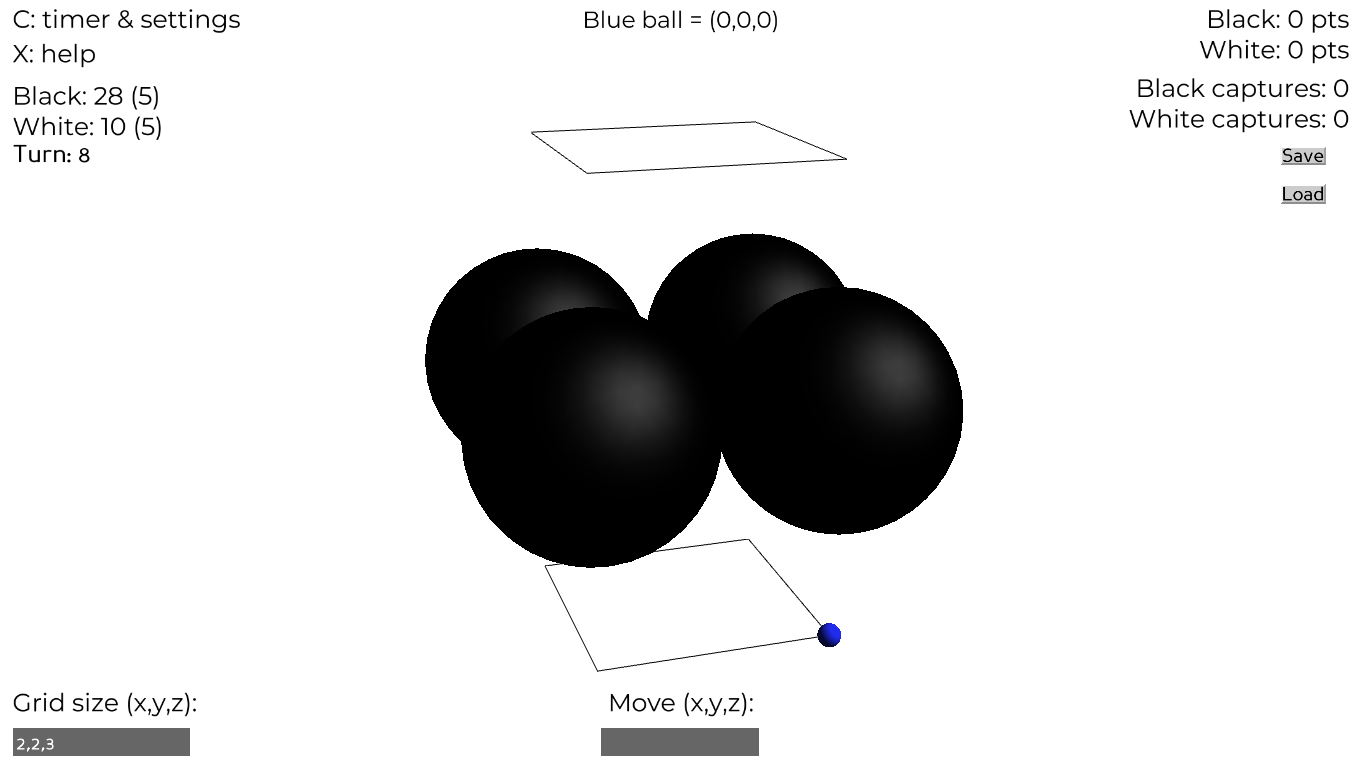
\includegraphics[width=\linewidth]{figures/baicontraej}
	\caption{Minimal counterexample to Bai's result. A two-dimensional black group possessing unconditional life on a \(2 \times 2 \times 3\) board.}
	\label{fig:baicontraejemplo}
\end{figure}	
	



%
%\vfill

%\section*{Glosario (Parte II)}
%\begin{center}
%	\begin{tabular}{p{2cm} p{4.7cm} p{2cm} p{4.7cm}}
	%		\toprule
	%		\textbf{Símbolo} & \textbf{Significado} & \textbf{Símbolo} & \textbf{Significado} \\
	%		\midrule
	%		$\partial R$ & Frontera de la región $R$ & $V$ & Región vital para un grupo \\
	%		$O$ & Ojo (región vital con un solo grupo frontera) & $U$ & Unión (región vital con más de un grupo frontera) \\
	%		$S,P$ & Conjunto de grupos del mismo color & $\Gamma$ & Juego de Go ($G,E,A,\Delta$) \\
	%		$\Delta$ & Función de transición del estado & $u_t$ & Estado del tablero en el turno $t$ \\
	%		\bottomrule
	%	\end{tabular}
%\end{center}
\clearpage